\PassOptionsToPackage{table}{xcolor}
\documentclass[11pt]{article}
%
%%%%%%%%%%%%%%%%%%%%%%%%%%%%%%%%%%%%
%% Common preamble
%%%%%%%%%%%%%%%%%%%%%%%%%%%%%%%%%%%%
% PAGE
\newcommand{\tuta}{\emph{T.~absoluta}}
\newcommand{\infest}{\rho}
\newcommand{\totinf}{\rho_{\mathrm{T}}}
\newcommand{\suitable}{\epsilon}
%% \usepackage{fullpage} % uncomment this when changing to jour/conf style
% FONTS
\usepackage{textcomp}
\usepackage{lmodern} % enhanced version of computer modern
\usepackage[T1]{fontenc} % for hyphenated characters and textsc in section title
\usepackage{xr}
\externaldocument[S:]{supplementary}
\usepackage{microtype} % some compression
\usepackage{times}
\usepackage{setspace} % For double line spacing
\doublespacing
\usepackage[left=1in,top=1in,right=1in,bottom=1in]{geometry}
\usepackage[pagewise]{lineno}
\linenumbers
\usepackage{marvosym}
%% \newcommand\wordcount{\immediate\write18{texcount -sub=section \jobname.tex  | grep ``Section'' | sed -e 's/+.*//' | sed -n \thesection p > 'count.txt'} (\input{count.txt}words)}
% MATH
\usepackage{amssymb}
\usepackage{mathtools} % contains amsmath which comes with align
\usepackage{amsthm} % newtheorem stuff
\usepackage{bm} % for bold math (use $\boldsymbol{}$)
% COLOR
\usepackage[usenames,dvipsnames]{color}
%%
% REFERENCING
% JM: Below is for affiliations
\usepackage{authblk}
% BIBLIOGRAPHY
\usepackage[square,sort&compress,numbers]{natbib} %sorts bibs when they are collectively cited
\usepackage[colorlinks=true,pdfborder={0 0 0},citecolor=RoyalBlue,linkcolor=black,urlcolor=Magenta]{hyperref}
\usepackage{cleveref} %%% IMPORTANT: cleveref comes before \newtheorem commands
   \crefname{figure}{Figure}{Figures}
   \crefname{table}{Table}{Tables}
   \crefname{theorem}{Theorem}{Theorems}
   \crefname{lemma}{Lemma}{Lemmas}
   \crefname{claim}{Claim}{Claims}
   \crefname{section}{Section}{Sections}
   \crefname{observation}{Observation}{Observations}
   \crefname{note}{Note}{Notes}
%%
% TABLES
\usepackage{multirow}
%% \usepackage{ctable} % provides toprule, bottomrule, midrule
\usepackage{array} % new implementation of tabular & array with lots of enhancements
%%
% FIGURES
\usepackage{graphicx}
\graphicspath{./figs}
\usepackage{grffile} % to set right names of files
%%
% CAPTIONS
\usepackage{caption}
\usepackage{subcaption} % supersedes subfigure & subfloat. try using options
%%
% LISTS
\usepackage{enumitem} %\begin{itemize}[leftmargin=*]
%% inline
\newlist{inline}{enumerate*}{1}
\setlist[inline]{before=\unskip{: }, itemjoin={{; }}, itemjoin*={{; and }}, label={(\roman*)}}
\usepackage{silence}
\WarningFilter{ctable}{Transparency disabled:}
\WarningFilter{xcolor}{Incompatible color}
% ALGO
\usepackage[ruled,linesnumbered]{algorithm2e}
%% comments & todo
\newcommand{\reportingCells}{\mathcal{C}_R}
\newcommand{\similarity}{\mathcal{S}}
\newcommand{\aacomment}[1]{({\color{magenta}AA: #1})}
\newcommand{\mmcomment}[1]{({\color{green}MM: #1})}
\newcommand{\tbcomment}[1]{({\color{blue}TB: #1})}
\newcommand{\mrccomment}[1]{({\color{red}MRC: #1})}
\newcommand{\jmcomment}[1]{({\color{cyan}JM: #1})}
\usepackage[colorinlistoftodos]{todonotes}
\newcommand{\TODO}[1]{\todo[inline,color=red!10,size=\small]{#1}}
%% COMMANDS
\newcommand{\comp}[1]{\overline{#1}}  %{\widetilde{#1}}
\DeclareMathOperator{\Var}{Var}
\DeclareMathOperator{\Cov}{Cov}
\DeclareMathOperator{\bigo}{O}
\DeclareMathOperator{\bigom}{\Omega}
\DeclareMathOperator{\davg}{d_{avg}}
\DeclareMathOperator*{\argmax}{arg\,max}
\DeclareMathOperator*{\argmim}{arg\,min}
% Note: \deg is already defined
\newcommand{\expect}{\mathbb{E}}
%
\newcommand{\ceil}[1]{\left\lceil #1 \right\rceil}
\newcommand{\floor}[1]{\left\lfloor #1 \right\rfloor}
%
\newcommand{\reals}{\mathbb{R}}
\newcommand{\field}{\mathbb{F}}
\newcommand{\integers}{\mathbb{Z}}
\newcommand{\pshort}{p_s}
\newcommand{\plocal}{p_{\ell}}
\newcommand{\pld}{p_{\ell d}}
\newcommand{\asd}{\alpha_s}
\newcommand{\afm}{\alpha_{\ell}}
\newcommand{\ald}{\alpha_{\ell d}}
\newcommand{\produce}{\mathrm{Prod}}
\newcommand{\veg}{\mathrm{V}}
\newcommand{\temp}{\mathrm{T}}
\newcommand{\consume}{\mathrm{Pop}}
\newcommand{\locality}{\mathrm{L}}
\newcommand{\export}{\mathrm{Export}}
\newcommand{\import}{\mathrm{Import}}
\newcommand{\process}{\mathrm{Proc}}
\newcommand{\moore}{\mathrm{M}}
\newcommand{\mooreRange}{r_\mathrm{M}}
%
\newtheorem{theorem}{Theorem}[]{\bfseries}{\itshape} 
\newtheorem{lemma}[theorem]{Lemma}{\bfseries}{\itshape}
\newtheorem{claim}[theorem]{Claim}{\bfseries}{\itshape}
\theoremstyle{definition}
\newtheorem{definition}[theorem]{Definition} % {\bfseries}{\itshape}
\newtheorem{observation}[theorem]{Observation} % {\bfseries}
\newtheorem{condition}[theorem]{Condition} % {\bfseries}{\itshape}
\newtheorem{note}[theorem]{Note} % {\bfseries}{\itshape}
% ROMAN NUMERALS
\makeatletter
\newcommand{\rmnum}[1]{\romannumeral #1}
\newcommand{\Rmnum}[1]{\expandafter\@slowromancap\romannumeral #1@}
\makeatother
%%
% TWO VERSIONS
%% \usepackage{etoolbox}
%% \newtoggle{withappendix}
%% \toggletrue{withappendix} % comment this if you want journal version
%% Usage: iftoggle{withappendix}{}{}
%%
%% math operator
%% \DeclareMathOperator{\sgn}{sgn}
% CODEBOX
%% \usepackage[framemethod=tikz]{mdframed}
%% \newmdenv[linecolor=black!10,innerlinewidth=0pt, roundcorner=4pt,innerleftmargin=6pt,
%% font=\ttfamily,innerrightmargin=6pt,innertopmargin=6pt,
%% innerbottommargin=6pt,backgroundcolor=black!10]{codeblock}
%%%%%%%%%%%%%%%%%%%%%%%%%%%%%%%%%%%%
%% preamble ends
%% from now on, draft specific
%%%%%%%%%%%%%%%%%%%%%%%%%%%%%%%%%%%%
%% \RequirePackage[l2tabu, orthodox]{nag}
\makeatletter
\renewcommand\AB@affilsepx{, \protect\Affilfont}
\makeatother
% Title on edge of suggested length
\title{Assessing the Multi-pathway Threat from Invasive Agricultural
Pests: Study of \emph{Tuta~absoluta} in Asia}
%% \title{A Multi-pathway Model to Assess the Threat of Invasive Agricultural
%% Pests: Case Study of \emph{Tuta~absoluta} in Asia}
\author[1]{Joseph~McNitt}
\author[2]{Young~Yun~Chungbaek}
\author[2]{Henning~Mortveit}
\author[2]{Madhav~Marathe}
\author[3]{Mateus~Ribeiro~de~Campos}
\author[3]{Nicolas~Desneux}
\author[4,5,6]{Thierry~Br\'{e}vault}
\author[7]{Rangaswamy Muniappan}
\author[2]{Abhijin~Adiga}
\affil[1]{Department of Mathematics, Virginia Tech}
\affil[2]{Biocomplexity Institute \& Initiative, University of Virginia}
\affil[3]{French National Institute for Agricultural Research}
\affil[4]{BIOPASS, CIRAD-IRD-ISRA-UCAD, Dakar, Senegal}
\affil[5]{CIRAD, UPR AIDA, F-34398 Montpellier, France}
\affil[6]{Universit\'{e} de Montpellier, CIRAD, Montpellier, France}
\affil[7]{Feed the Future Integrated Pest Management Innovation Lab}
\date{}
\setcounter{Maxaffil}{0}
\renewcommand\Affilfont{\itshape\small}

\begin{document}
\maketitle

\begin{abstract}
Modern food systems facilitate rapid spread of pests and pathogens.
Understanding their dynamics is critical to better prepare for emerging
invasions. We modeled the multi-pathway spread of an invasive species as a
propagation process over a time-varying network that accounts for
biology, seasonal production, trade and demographic information. This
generic data-driven approach was applied to study the spread of a
devastating pest of tomato \emph{Tuta absoluta}, in South and Southeast
Asia -- a region at the frontier of its current range. Analysis with
respect to historical invasion records in Bangladesh suggests that even
with modest self-mediated spread capabilities, the pest can quickly expand
its range through domestic city-to-city vegetable trade. Tomato imports and
exports in the region were analyzed to  assess the possible routes of
introduction, and we predicted the spread pattern in the rest of the study
region. There is a strong chance that within five to seven years \tuta{}
will invade all major vegetable growing areas of Mainland Southeast Asia if
no steps are taken to mitigate the spread. Further, we showed that
monitoring and effective interventions in major production areas could
greatly reduce the speed of the spread.
\end{abstract}
%%
\section{Introduction}

somewhere say that it is not clear what its flying capacity is

say modeling multiple countries requires lot more data

make sure intro has challenges

model, data uncertainty, pathway models, talk about Douma et al.

%%  which has invaded more than 60\% of
%% tomato producing land over the last decade.

As international trade intensifies, no region is spared from the threat of
exotic species invasions~\cite{hulme2009trade}. Once introduced, with few
restrictions in place, domestic trade facilitates their rapid spread within
a country~\cite{}. Climate change and detrimental impact of intensive
agriculture on natural resources are likely to further aggravate this
problem~\cite{early2016global}.  Models play an important role in
(i)~discerning the roles of different pathways from one
another~\cite{13challenges}; (ii)~predicting the spatio-temporal spread
under different scenarios of introduction and intervention strategies; and
(iii)~exposing gaps in data and understanding of the phenomenon. However,
impending invasions of agricultural pests present difficult hurdles.
Accounting for multiple drivers of dispersal (ecological suitability,
production, trade, etc.) tends to make the model complex and demands
multi-disciplinary research. At the same time, we are presented with the
challenge of data inadequacy, which makes it nearly impossible to calibrate
and validate these models. Few and often inaccurate incidence reports, lack
of production and trade data, and limited understanding of the pest's
biology are some examples. This problem is acute when the study region is
data poor. Further, if the region is comprised of multiple countries, one
has to account for the heterogeneity of data; multiple sources, different
formats and resolution. There is an urgent need for robust methods that can
provide useful models with limited data.

Pest risk maps have evolved ... long-term establishment. 
 We developed a 

%% The world is witnessing a rapid increase in trade and
%% travel~\cite{ercsey2012complexity}. Due to this increased connectivity,
%% both international and domestic, no region is spared of the threat from
%% exotic species invasion~\cite{hulme2009trade}.   As a result, global food
%% security, human health and social welfare will be adversely impacted.

The South American Tomato leafminer, or \emph{Tuta absoluta}, a pest of the
tomato crop, is a representative among the recent biological invasions that
have significantly perturbed global food production. Indigenous to South
America, \tuta{} was accidentally introduced to Spain in~2006, and since
then it has rapidly spread throughout Europe, Africa, Western and Central
Asia, the Indian subcontinent, and parts of Central
America~\cite{desneux2010biological,biondi2017}. With tomato being a
commercially important crop, this invasion has had significant global
impact~\cite{campos2017western}. In the Netherlands and Turkey alone, the
annual estimated intervention cost are \EURdig4 million and \EURdig167
million per year~\cite{}, respectively. It is well accepted that trade
played a critical role in \tuta{}'s rapid spread. On multiple occasions it
has been discovered in packaging stations and its spread pattern is
correlated with prime trade routes~\cite{karadjova2013tuta}. 

%% The wide-spread
%% adoption  of green houses and tunnel farming have allowed it to overwinter
%% as well as survive the wet season. 
%% There is a great need to understand the
%% dynamics of this pest in order to predict its future invasion pattern, and
%% design effective prevention and mitigation policies.

%% Due to extensive insecticide
%% treatment in Europe, insecticidal resistance has been recently observed in
%% populations~\cite{guedes2013tomato}. 
%% Overall,
%% lack of effective indigenous predators has made integrated pest management
%% (IPM) a challenging task.
%%~\cite{potting2013tuta,oztemiz2014tuta}

%% Since tomato is among the top two traded vegetables in the
%% world\footnote{\url{http://www.fao.org}}, 

%% Faced with the challenging task of preparing for the invasion of pests and
%% pathogens, and responding effectively to mitigate such incursions should
%% they happen, decision makers are increasingly relying on  computational
%% models of pest risk maps and spread to aid decision
%% making~\cite{venette2010}.  While models that create pest risk maps (e.g.
%% CLIMEX) are useful to identify locations which are suitable for long-term
%% establishment, % and cause harmful impact spread models help specify the
%% spatio-temporal dynamics of how the pest spreads.  The latter approach is
%% particularly useful in planning for the possible threat from an invasive
%% species~\cite{perrings2014merging,barbier2013implementing,paini2010threat,paini2010threat,paini2016global}
%% through {\it in silico} experiments simulating hypothetical invasion
%% scenarios. 
%% Together, these tools can be used to address questions such as
%% which locations to monitor, what control measures to take (areawide IPM
%% practices, trade restrictions, etc.), what is the impact on the economy and
%% health, and so on. 

We describe a multi-pathway propagation model 
to study the spread of \tuta{} in the region of South
and Southeast Asia comprising of 10 countries: members of the Association
of Southeast Asian Nations (ASEAN) and Bangladesh. To develop this model,
we identified, analyzed, and fused disparate datasets corresponding to
ecology,  
%% (temperature, precipitation, elevation, vegetation, host
%% plant presence), 
%% (host preference, suitability, population growth),
production, trade 
%% (imports, exports, domestic trade, city locations, city to city distances), 
and demographic factors. 
%% (per capita consumption and population). 
Learning methods such as Classification and Regression Trees
(CART)~\cite{breiman2017classification} and Random Forests were used for
parameter space exploration and sensitivity analysis.  To our knowledge,
this is the first study that explicitly considers multiple pathways of
introduction and spread of \tuta{}.  Earlier modeling efforts have only
accounted for ecological aspects and self-mediated
spread~\cite{desneux2010biological,tonnang2015identification,guimapi2016modeling}.
A major hurdle in modeling spread of emerging pests and pathogens in data
poor regions is the lack of accurate incidence reports, production and
trade dynamics. To fill these gaps we gathered quantitative and
qualitative information from more than 50 research articles and reports
that analyze vegetable production in the region.

%% This problem is compounded in data-poor regions due to
%% unavailability and inaccessibility of data on production and trade, making
%% parameterization and validation nearly impossible. 
%% For
%% parameterization and sensitivity analysis of this complex model, we used a
%% Classification and Regression Trees approach~\cite{lamperti2018agent}.


This is a timely and important study for several reasons. In the recent
years, there has been a thrust to improve vegetable production in all the
countries of this region~\cite{ali2001}. With the pest having
already spread to major tomato producing areas in
Bangladesh~\cite{hossain2016first}, there is a high chance that it will be
introduced to the remaining countries in the near future. Such invasions
can have devastating effect on the economy and livelihood of farmers.
Moreover, invasion in Mainland Southeast Asia in particular is a serious
threat to China, the largest producer of tomato, and Australasian
neighbors.

%% Furthermore, no earlier work has studied the entire
%% Southeast Asia region, particularly in the context of agricultural crops.

\paragraph{Summary of results.} 

consumption areas

%% We studied \tuta{} invasion of Bangladesh using the proposed model. 
Our analysis with respect to historical invasion records indicate two
possibilities of spread of \tuta{} in Bangladesh, one where trade is the
dominant pathway and the other where it is not. In particular, even with
slow self-mediated dispersal, the pest could have rapidly expanded its
range aided by domestic tomato trade.  There is also a possibility of
multiple introductions of the pest to this country. For the rest of the
study region our models predict a faster southward spread to Thailand,
Malaysia and Singapore than eastward spread in Mainland Southeast Asia due
to higher trade activity in the former region. Country specific analysis
shows that once introduced to a major production area, the pest will spread
all over the country within two to three years. However, gaps in data and
understanding of trade interactions between countries makes it difficult to
predict pest movement between countries. We also demonstrated the efficacy
of intervening at the trade level; quarantining few key production areas
can contain the spread or significantly reduce the spread rate.

%%
\section{Methods}
%%
\paragraph{Data.} The global datasets used in the model and for analysis are
described in Table~\ref{S:tab:data} of the supplement. Country specific data on
seasonal production, consumption, processing and trade was
obtained from websites of agriculture ministries, research articles and technical
reports (Table~\ref{S:tab:countryData} in SI). Almost
all the datasets used are openly available. Some information was
provided by local contacts in Bangladesh (for e.g., \tuta{} incidence
reports in Table~\ref{S:tab:bgdData}), Vietnam and Cambodia.
%%
\paragraph{\tuta{} biology.}
The tomato leafminer exhibits a short life cycle of about 24--38 days
(temperature at $25\pm3^\circ$C), from egg to adult, as it is a
multivoltine species with overlapping generations in the
field~\cite{guedes2012tomato}. This species causes serious damage to
numerous solanaceae crops such as eggplants, potatoes, and especially
tomato crops~\cite{sylla2018}. It penetrates into tomato leaves, stems, or
fruits, wherein it feeds and develops by creating conspicuous mines as well
as galleries. \tuta{} additionally restricts tomato plant growth by feeding
on the growing tips. Considering the warm weather throughout the year,
particularly in the dry season, the study region presents ideal conditions
for rapid development and spread of \tuta{}. Pest risk
analysis~\cite{tonnang2015identification} shows that the Ecoclimatic Index
for this region is above~$50$ (highly suitable). Spatial distribution
assessment survey of \tuta{} eggs has shown its high dispersive capacity in
tomato producing areas~\cite{martins2018assessing}. The dispersion in a
tomato cultivation starts mainly at the periphery and
the pest is able to migrate between tomato farms to generate egg aggregation at the
crop edges. The pest spread behavior among seasonal crop resources
is often non-random and directional~\cite{martins2018assessing}.
Sylla~et~al.~\cite{sylla2018} analyzed host preference of~\tuta{} in France
and Senegal. While the highest preference is for tomato, it can survive
well on eggplant and potato, which happen to be major vegetable crops in
the study region. However, since \tuta{} primarily attacks leaves of
eggplant and potato, the chance of the pest spreading through trade of
these crops seems to be low.
%%
%% Each cell~$v$ has the following time varying attributes: \aacomment{these
%% are not necessary: NDVI~$\veg(v,t)$,
%% temperature~$\temp(v,t)$,} monthly production of preferred host crops and
%% consumption~$\consume(v,t)$, where~$t$ corresponds to a month.
%% \aacomment{This should get into Tonnang discussion: Since NDVI
%% data is available at a much finer resolution (see Table~\ref{tab:data}),
%% for each cell, we assign the maximum of the NDVI data points that fall in
%% this cell for that month.} For production, we consider the following
%% vegetables: tomato, potato, eggplant in metric tonnes (see
%% Section~\ref{sec:biology} on choice of host crops). Annual country-level
%% production data (in volume) is spatially disaggregated using SPAM data
%% on spatial distribution of vegetable production. \aacomment{needs
%% explanation. statistical analysis should come here}. Further, for each cell,
%% this production was distributed temporally-- one value for each month of
%% the year. We observed that precipitation is a primary driver of production
%% in the study area; during wet months, the amount of production is
%% considerably less. \aacomment{statistical analysis should come here} (See Supplementary Information).
%% \aacomment{pending: consumption, import/export}

%%
\paragraph{Multi-pathway spread model.} We developed a stochastic
propagation model to simulate the multi-pathway spread of~\tuta{}.  Key
concepts are illustrated in Figure~\ref{fig:concept}.
The study region is
divided into cells by overlaying a grid
(0.25\textdegree~$\times$~0.25\textdegree). Each cell is in one of the
three states: susceptible ($S$) denoting pest free state, exposed ($E$)
denoting that the pest has been introduced but the population has not yet
built up to influence other cells, and infectious ($I$) denoting that the
pest has established and the cell can influence its neighbors. The cell
states are updated in discrete time steps, where each step~$t$ corresponds
to a month.  The probability that a cell~$v$ transitions from state~$S$
to~$E$ is determined by (i)~suitability of the cell for \tuta{} to
establish at that time step~$\suitable(v,t)$ and (ii)~influence of
``neighboring'' cells in state~$I$ depending on the pathway. An exposed
cell transitions to state~$I$ after a latency period of~$\ell$ time steps.
This is the time required for the population to build up to infect other
cells.  Once the pest has established in a cell, the cell remains infected
forever, a fair assumption considering that, historically, eradication of
\tuta{} has not been successful\footnote{The only exception is United
Kingdom where the pest was detected early and
eradicated~(\url{https://gd.eppo.int/reporting/article-340}).}.  The
infectiousness of a cell~$\infest(v,t)$ is modeled as a linear function of
host presence at time~$t$, for which we use the weighted sum of production
volume of tomato, eggplant, and potato in that cell at time~$t$. The
weights correspond to relative carrying capacity of \tuta{} on the three
hosts~\cite{sylla2018}.

%%
\begin{figure}[t]
\centering
\begin{subfigure}[b]{.4\textwidth}
    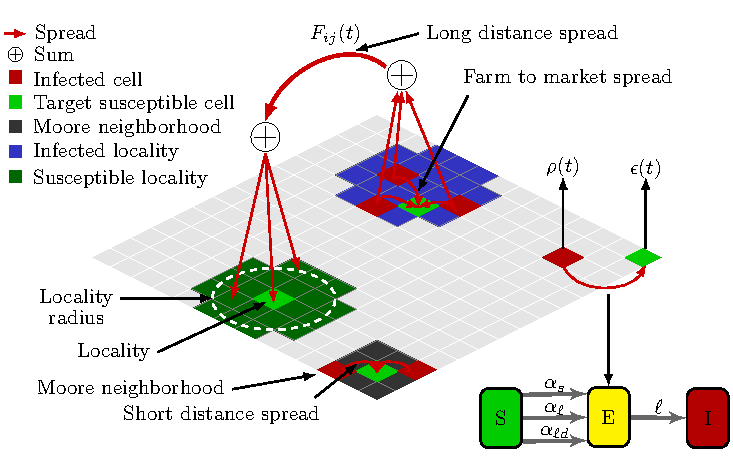
\includegraphics[width=1.1\textwidth]{figs/model_schematic.pdf}
\caption{\label{fig:concept}}
\end{subfigure}
%%
\begin{subfigure}[b]{.56\textwidth}
    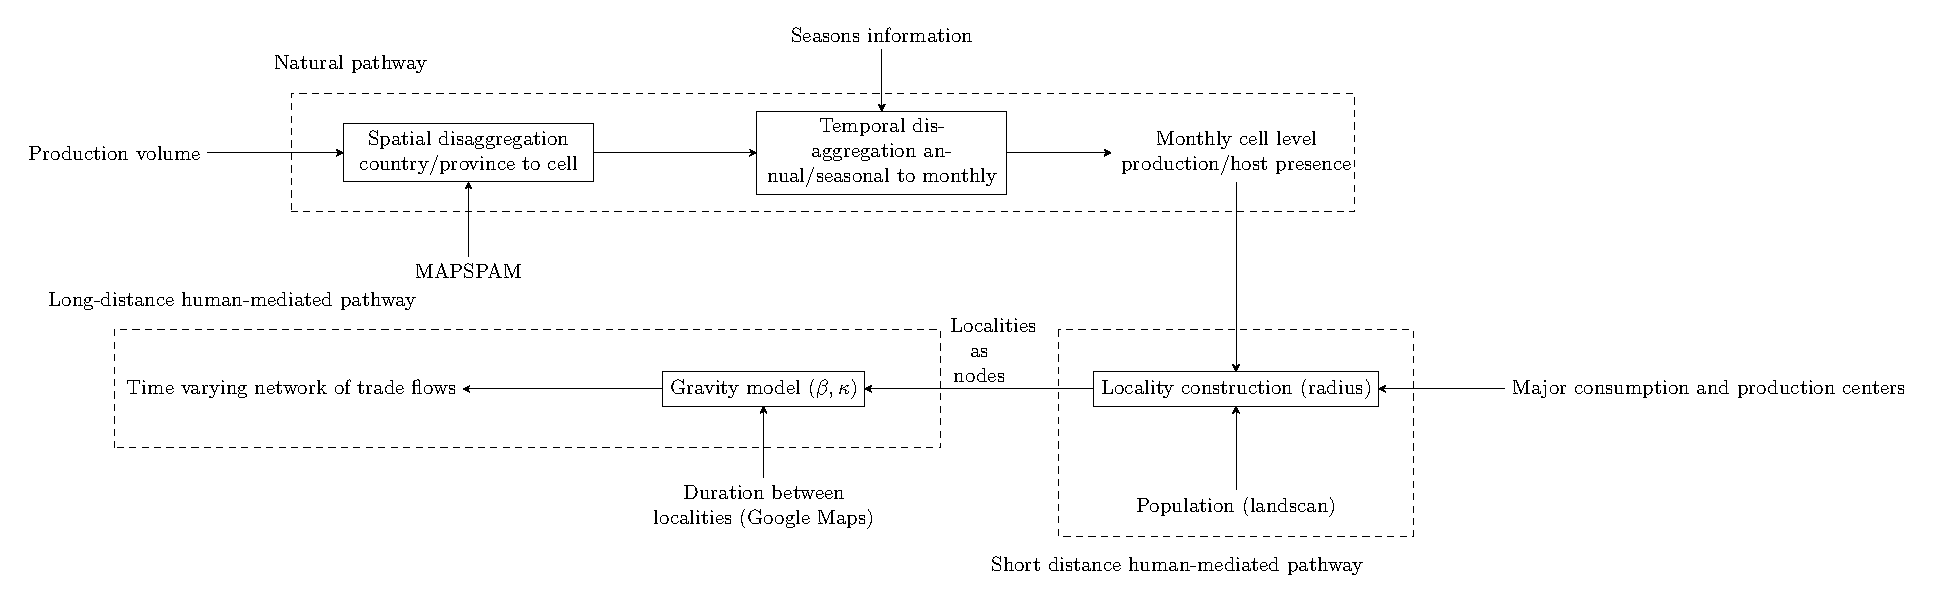
\includegraphics[width=1.05\textwidth]{figs/pipeline.pdf}
\caption{\label{fig:pipeline}}
\end{subfigure}
\caption{\textbf{The multi-pathway model.} (a)~The network structure,
pathways and dynamics are captured in the illustration.
%% , which is
%% approximately~$27.8\mathrm{km}\times\mathrm{27.8km}$ at the equator. 
%% These
%% dimensions are comparable to that used in the cellular automata model of
%% Guimapi~et.~al.~\cite{guimapi2016modeling} ($25\mathrm{km}\times25\mathrm{km}$). Details of locality construction are in Section~\ref{S:sec:locality}. 
%% Long distance human-mediated dispersal is modeled
%%las the spread between localities through. 
Also shown are the states and factors
that influence state transitions: infectiousness of a neighbor, suitability
of the cell for pest establishment, pathway parameters and latency period.
\label{fig:modelConcept}
(b)~\textbf{Pipeline.} The process of constructing the spatio-temporal
network of cells is outlined. Key modules are highlighted along with 
input data.}
\end{figure}
%%

There are three pathways by which a cell can become infected:
short-distance dispersal, local human-mediated dispersal and long-distance
dispersal. Short-distance dispersal captures the spread through natural
means; from an infested cell to cells in its Moore neighborhood of
range~$\mooreRange$.
The probability that a susceptible cell gets exposed (E) at time step~$t$
through short-distance spread is as follows:
%%
\begin{linenomath}
\begin{align}\label{eqn:pshort}
    \pshort(v,t)=\suitable(v,t)\bigg(1-
    \exp\Big(-\asd\sum_{v'\in\moore_v(\mooreRange)}\infest(v',t)\Big)\bigg),
\end{align}
\end{linenomath}
%%
The probability depends on the suitability of the cell~$\suitable(v,t)$,
infestation level of each neighboring cell in the Moore neighborhood with 
range~$\mooreRange$,~$\infest(v',t)$ and the scaling factor,~$\asd$, which is the transmission rate for this pathway. The
function form is explained in Section~\ref{S:trans}.

For human-assisted spread we identified large urban areas in the region
which we refer to as {\it localities} (Figure~\ref{fig:modelConcept}) and
considered 
interactions within and between localities. These areas act as attractors
of vegetable flows due to high consumption or production and house the necessary
infrastructure: wholesale markets, traders and distributors.
%% Also, since horticultural products are less
%% durable, owing to lack of good storage and transport
%% infrastructure~\cite{ali2001}, typically, much of the major producing
%% regions are close to cities~\cite{buckmaster2014going}. Only a cell
%% belonging to a locality is affected by the human-mediated pathways. 
Each
\emph{locality} consists of all grid cells which are within a certain
distance (determined by \emph{locality radius}) from its corresponding center. Local
human-mediated dispersal is modeled as the spread between cells
belonging to a locality.
%% Since local
%% farm--market dynamics are hard to model~\cite{rebaudo2011}, we used a
%% simple approach.
%% For a cell in a locality (say~$L$), its neighbors are all cells that belong
%% to the locality.  
%% The objective is to cell's state is influenced by the infected cells in
%% its locality through the marketing chain.  In general, it is hard to model
%% the local dynamics as there are several actors in bringing the commodities
%% from farm to market to consumers.  Further, these are country and commodity
%% specific.  See for example Kethonga~et~al.~\cite{kethonga2004} for the
%% typical structure of marketing chains and Rebaudo~et~al.
%% for modeling human interactions in the context of invasive species spread.
%% Here, we use a simple approach. 
Every cell~$v$ is influenced by cells in
its locality~$\locality$ based on their infectiousness.  The expression is
similar to that in~\eqref{eqn:pshort}, but with cells in the locality
instead of the Moore neighborhood.
%%
\begin{align}\label{eqn:plocal}
    \plocal(v,t)=\suitable(v,t)\bigg(1-
    \exp\Big(-\afm\sum_{v'\in\locality}\infest(v',t)\Big)\bigg),
\end{align}
%%
where~$\afm$ is the scaling factor. The details of
locality construction are provided in Section~\ref{S:sec:locality} of SI.

Long-distance human-mediated dispersal corresponds to spread through trade
between localities. For this purpose, we considered only tomato trade as
there is not much evidence of \tuta{} spreading through trade of other
hosts. We modeled domestic trade using a gravity model approach accounting
for tomato production, processing, imports and exports in each locality and
the travel time between localities. 
%% However, this information was accounted for in experiment
%% design to identify possible starting locations or ``seeds'' for each
%% country.  
The probability of spread is directly proportional to the trade
flow~$F_{ij}$ from one locality ($i$) to another ($j$).
%% \paragraph{State transitions.} The rules for state transitions are shown in
%% Figure~\ref{fig:SEI}. A susceptible ($S$) cell can be influenced by
%% infectious (state~$I$) cells through the three different pathways. Each
%% such cell infects the susceptible cell with some probability. If \tuta{} is
%% succesfully introduced to a cell, it moves from state~$S$ to~$E$. The
%% exposed state corresponds to the situation where \tuta{} has established,
%% but it is not widespread in the area to influence other cells. It stays in
%% state~$E$ for one time step before transitioning to state~$I$. This is a
%% reasonable assumption considering that the conditions are favorable for the
%% pest to complete a life cycle within one month. 
%%
%% \begin{figure}[ht]
%%     \centering
%%     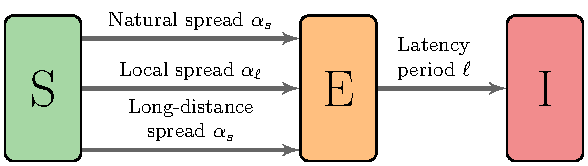
\includegraphics[height=.16\textwidth]{figs/SEI.pdf}
%%     \caption{Schematic of the SEI process.\label{fig:SEI}}
%% \end{figure}
%%
%% 
%% \paragraph{Susceptibility and infectiousness of a cell.} We have used
%% monthly production to determine the susceptiblity of a cell in state~$S$
%% and infectiousness of a cell in state~$I$. The suitability of a cell~$v$
%% for pest establishment at time~$t$ is denoted by~$\suitable(v,t)$. This
%% is~$1$ if production at~$t$ is non-zero and~$0$ otherwise.  For a cell in
%% state~$I$, the level of infestation in an infected cell~$v$ at time~$t$ is
%% denoted by~$\infest(v,t)$. It is modeled as a linear function of host
%% presence at time~$t$, for which we use the weighted sum of production
%% volume of tomato, eggplant, and potato in that cell
%% at time~$t$. The weights correspond to relative oviposition preference of
%% \tuta{} on the three hosts.
%% 
%%
Suppose cell~$v$ belongs to locality~$i$. Then, the probability of cell~$v$
transitioning from~$S$ to~$E$ due to long-distance dispersal is given by:
%%
\begin{linenomath}
\begin{align}\label{eqn:plocal}
    \pld(v,t)=\suitable(v,t)\bigg(1-
    \exp\Big(-\ald\sum_{j\ne i}\sum_{v'\in\locality(j)}F_{ji}\infest(v',t)\Big)\bigg),
\end{align}
\end{linenomath}
%%
where~$\ald$ is the scaling factor.
The model parameters and their values are summarized in
Table~\ref{tab:param}. 
%%
\begin{table}[t]
\caption{Model parameters and their values.\label{tab:param}}
    \centering
	\small
\rowcolors{2}{white}{gray!15} % For this to work, put \PassOptionsToPackage{table}{xcolor} before \documentclass
    \begin{tabular}{p{.093\textwidth}p{.33\textwidth}p{.5\textwidth}}
    %{cp{.25\textwidth}p{.25\textwidth}lr}
		\hline		
		Parameter & Description & Value/range \\
\hline		
\hline
$\mooreRange$ & Range of Moore neighborhood & $\{1,2,3\}$ corresponding to
spread per month of 
approximately~$25$kms,~$50$kms and~$75$kms
respectively~\cite{guimapi2016modeling,martins2018assessing}. \\
%% $\suitable$ & Suitability threshold \\
$\ell$ & Latency period to transition from $E$ to $I$ & $\{1,2,3\}$ months
based on time for the pest to complete life cycle (\tuta{} biology in
Methods). \\
Monthly production & Disaggregation of annual production to monthly values
& \emph{Uniform} throughout the year or \emph{seasonal} based on regression
analysis (Methods). \\
$\beta$ & Gravity model distance function exponent & $\{0,1,2\}$ \\
$\kappa$ & Gravity model distance function cut-off & Between $4$ to $16$ hours
of travel time. \\
Seed & Location and time of initial infestation & Scenarios based on
countries (Table~\ref{S:tab:seed})\\
Locality radius & Determines cells assigned to a locality & 100kms \\\hline
$t_s$ & Time step of initial infestation & $\{3,4,5\}$ corresponding
to March, April and May respectively based on first report in
Bangladesh~\cite{hossain2016first}. \\
%% $\infest$ & Infectivity of a cell based on amount of production & \\
$\asd$ & Short-distance spread scaling factor & In the interval $[0,500]$.\\
$\afm$ & Local human-mediated dispersal scaling factor & In the interval $[0,500]$.\\
$\ald$ & Long distance spread scaling factor & In the interval $[0,500]$.\\
\hline
\end{tabular}
\end{table}
%%
\paragraph{Network construction.} 
Figure~\ref{fig:pipeline} provides a schematic of the network construction.
The first step was to estimate monthly production volume of tomato,
eggplant and potato for each cell. First, we estimated annual production in
each cell followed by disaggregation to monthly production. The annual
production was estimated using the vegetable production available at the
highest resolution for each country (at the level of province to just one
value for the entire country) and a synthetic dataset called Spatial
Production Allocation Model (SPAM)~\cite{spam}.
Gathering qualitative data from multiple sources, we inferred that the
cropping pattern in this region depends primarily on two factors:
seasons--dry and wet, and elevation--highland (upland) and lowland. Also,
barring few exceptions, the production of the considered host crops peaks
in the winter and is lowest during the rainy season (monsoon).  To predict
seasonal production, we used linear regression to model the production rate
as a function of precipitation, temperature, and elevation. Regional tomato
and eggplant production data is available for Philippines.
%% For each region, we obtained the product rate by
%% normalizing quarterly production values with respect to maximum value among
%% these. We used production rate instead of production values since there are
%% several factors that determine a region's production: climate, vegetable
%% preference, demand, etc.  Therefore, it may not be meaningful to compare
%% production across regions.  
%% We conducted a linear regression with the
%% product rate as a dependent variable and precipitation and temperature and
%% elevation as independent variables.  To control elevation, we classified
%% the elevations into two groups, high and low, using $k$-means clustering
%% (SPSS~24.0). Due to the small sample size, we excluded the samples in the
%% high-elevation group and conducted a linear regression analysis for the
%% group of low elevation~($< 235$ masl). 
The regression results showed that
precipitation was a statistically significant
predictor ($p <0.001$). For validation, the regression function was
applied to locations of different countries where this information is
available and visually compared. More details on the methods and validation are
provided in Section~\ref{S:sec:prod}. 
%% There is very little data
%% available for validation. Most of the data is qualitative, just providing
%% information on growing and harvesting months. The regression function was
%% applied to locations of different countries where this information is
%% available and visually compared.  More details of the methods, country
%% specific data and challenges in this regard are covered in
%% Section~\ref{S:sec:prod}. The infectiousness of cell~$v$ at
%% time~$t$,~$\infest(v,t)$ is the production at~$t$, while its
%% suitability,~$\epsilon(v,t)$ is~$0$ if~$\infest(v,t)=0$ and~$1$ otherwise.
%% on data availability. The first method was used if only seasonal
%% production is available for a region or country. In this case, we first
%% estimated seasonal production in each cell and then disaggregated it
%% to obtain monthly production. Here, due to unavailability of data for tomato and eggplant, we used SPAM's total
%% vegetable production as surrogate. To disaggregate into monthly production,
%% we studied the relationship between production, precipitation, and elevation.
%% For lowland areas, %(elevation less than ???) 
%% production is negatively
%% correlated with precipitation ($r<-0.75$).

%% \paragraph{Network structure.} The resulting network consists of~$8,010$
%% cells and~$109$ localities.  
%%
%%
%% \begin{table}[t]
%%     \caption{Model parameters and variables, their ranges and references.\label{tab:data}}
%%     \centering
%% 	\small
%%     \begin{tabular}{l p{4cm} p{3cm} p{5cm}}
%%     %{cp{.25\textwidth}p{.25\textwidth}lr}
%% 		\hline		
%% 		Parameter & Description & Range/values & Source \\
%% \hline		
%% \hline
%% $\mooreRange$ & Range of Moore neighborhood & 1,2,3 &
%% \cite{guimapi2016modeling}\\
%% $\ell$ & Latency period to transition from $E$ to $I$& 1,2,3 & \\
%% \hline
%% $\beta, \kappa$ & Gravity model parameters & 300--500,2 &
%% \cite{venkatramanan2017towards}\\
%% -- & Locality population threshold and radius & 250,000, 100kms &
%% population of cities~\cite{citypop} and reports\\
%% \hline
%% $\suitable$ & Suitability threshold & 0\\
%% $\infest$ & Infectivity of a cell based on amount of production & & Host
%% production (SPAM), host preference~\cite{sylla2018}, precipitation and
%% elevation \\
%% \hline
%% Scenarios & Seeding simulations: time and cells to infect & 4 cases:
%% Bangladesh (B1 and B2), Malaysia (M1) and Philippines (P1) & \tuta{} incidence
%% reports in Bangladesh, FAOSTAT for international trade and migration
%% reports.\\
%% Start month & & March, April, May & Based on incidence reports\\
%% \hline
%% $\asd$ & Short-distance spread scaling factor & 0--500\\
%% $\afm$ & Local human-mediated dispersal scaling factor & 0--500\\
%% $\ald$ & Long distance spread scaling factor & 0--500 \\
%% \hline
%% \end{tabular}
%% \end{table}
%%

We modeled the flow of fresh tomato crop between markets based on the following
assumptions: (i)~The total outflow from a city depends on the amount of
produce in its surrounding regions and imports from countries outside the
focus region at time~$t$, and (ii)~the total inflow depends on total
consumption, processing demand, and exports from the city to countries
outside the focus region. While there is strong evidence of tomato trade as
a possible pathway of \tuta{} spread~\cite{biondi2017}, there is no
evidence of a similar role of eggplant or potato trade. Hence, we modeled
only tomato trade. For each country, the domestic flow is estimated using a
doubly constrained gravity
model~\cite{kaluza2010complex}. For a city~$i$,
let~$O_i$ and~$I_i$ denote total outflow and total inflow respectively, and
$\locality(i)$ denotes all cells which are assigned to it.
The flow~$F_{ij}$ from city~$i$ to city~$j$ is given by
%%
\(
   F_{ij}(t)=a_i(t)b_j(t)O_i(t)I_j(t)f(d_{ij}),
\)
%%
where, $d_{ij}$ is the time to travel from~$i$ to~$j$, and $f(\cdot)$ is
the \emph{distance deterrence function}:
$d_{ij}^{-\beta}\exp(-d_{ij}/\kappa)$, where~$\beta$ and~$\kappa$ are
tunable parameters. The
coefficients~$a_i$ and~$b_j$ are computed through an iterative process such
that the total outflow and total inflow at each node agree with the input
values~\cite{kaluza2010complex}. Overall, we have~12 networks
representing flows for each month. The outflows and inflows are calculated
as follows:
%%
\begin{align}\label{eqn:flow}
    O_i(t)&=\produce(i,t)+\import(i,t)-\export(i,t)-\process(i,t),\\
    I_i(t)&=\consume(i)\,.
\end{align}
%%
Here,~$\produce(i,t)$ is the monthly production and~$\consume(i)$ is the
population of the locality as a surrogate to consumption. The latter is the
sum total of population in every cell that belong to the locality.
$\export$ and ~$\import$ are the monthly total export to and import from
outside the country respectively. $\process(i,t)$ is the tomato produced
for processing. Since for this purpose tomato is typically cultivated and
consumed locally, we subtract this volume from the outflow.
Country-specific details of how locality attributes were estimated is in
Section~\ref{S:sec:locAttrib}.
%% We did not incorporate international trade as the volume is negligible compared to
%% domestic production with the exception of trade between Malaysia and Singapore. 
%% More details in this regard are provided in Section~\ref{S:sec:locAttrib}.
Since no data is available on volume of trade between markets, to validate
the modeled trade networks, we gathered
qualitative information from reports and research articles which show
evidence of tomato or vegetable flow between market pairs. The results of
this analysis is in Section~\ref{S:sec:tradeFlows}.

Trade between countries of the focus region was not modeled as there is no
adequate information on ports of entry or monthly flow volumes. However,
they were accounted for to determine possible routes of entries and in
turn, to seed the simulations. However, there is one exception. We included
Singapore as a locality of Malaysia while applying the gravity model due to
high trade and mobility between the two countries.  case -- Malaysia to
Singapore -- by including the latter as a locality of Malaysia and applying
the gravity model. While most of the other flows were minor in comparison
to domestic flows, major flows that were ignored were from Thailand and
Vietnam to Malaysia.
%% Since
%% there is lot of interaction between the two countries, weMalaysia and Singapore
%% was included Malaysian

\paragraph{Parameterization and experiment design.}
The goodness of fit of a parameter instance was determined by comparing the
simulation output with \tuta{} incidence reports. We have incidence
information from eight locations in Bangladesh where pheromone traps were
installed (Figure~\ref{fig:bgdClassA} and Table~\ref{S:tab:bgdData}). The
spread was simulated with infestation starting from the location of first
report (Panchagarh, Bangladesh). For each cell, empirical probability that
it is in state~$I$ at time~$t$ was computed (averaged over 100
repetitions). The output was compared with ground truth using a similarity
function adapted from~\cite{carrasco2010unveiling}.  Let~$v$ be a reporting
cell and~$t_v$ denote the month of actual report of pest presence.  To
account for uncertainty in reporting, we consider a time
window~$U_\tau=[t_v-\tau,t_v+\tau]$ during comparison, where~$\tau$ is the
uncertainty parameter. We set~$\tau=2$, i.e., error within $\pm2$ months is
tolerated.  Supposing~$\reportingCells$ is the set of cells corresponding
to ground truth,  and ~$p(v,t)$ is the empirical probability that cell~$v$
is infected at time~$t$ in the model, then, the similarity~$\similarity$ is
given by,
%%
\begin{linenomath}
\begin{align}\label{eqn:similarity}
    \similarity=\sum_{v\in\reportingCells} \Big(\sum_{t\in U_\tau}p(v,t)
    + \sum_{t\notin U_\tau}\big(1-p(v,t)\big) \Big)\,.
\end{align}
\end{linenomath}
%%
Therefore, the maximum possible value
of~$\similarity$ is~$8$ (exact match with ground truth) and minimum is~$0$.

The range or values of model parameters are in Table~\ref{tab:param}.
Parameter space exploration was conducted in multiple iterations.  First,
we coarsely sampled the space. With model parameters as independent
variables and the goodness of fit measure defined in~\eqref{eqn:similarity}
as the dependent variable, we used Classification and Regression Trees
(CART) approach to identify subspaces for which similarity score was high
and rejected subspaces for which similarity was low. Based on this, in the
subsequent phases, we refined our search to improve the parameterization.
More details of the CART analysis is presented in Section~\ref{S:sec:cart}.
Simulations were performed on more than~$500,000$ parameter combinations
using a high performance computing cluster.

%% In the second phase,
%% we applied the select models from the previous phase to the rest of the
%% region to study how various conditions affect the nature and rate of
%% spread: different pest introduction scenarios, seasonality of production
%% and trade, and interventions or the lack thereof.
%% 
%% re

\paragraph{Analysis of spread pattern}
To analyze the spread patterns of selected models from the parameterization
phase, the simulation outputs were clustered using X-means
algorithm~\cite{pelleg2000x,andrei_novikov_2018_1491324}, an extension of
the classical K-means algorithm. It uses Bayesian information criterion to
estimate the optimal number of clusters. The simulation outputs (time and
cell indexed empirical probabilities) were clustered based on Euclidean
distance. To discover the relationship between spread pattern and model
parameters, clusters were further analyzed using CART with model parameters
as independent variables and the cluster index as the dependent variable.
Note that model parameters played no role in clustering process.
Figure~\ref{fig:clusterOutline} outlines the entire process.

biases in spread pattern and number of clusters
%%
\begin{figure}[b]
    \centering
    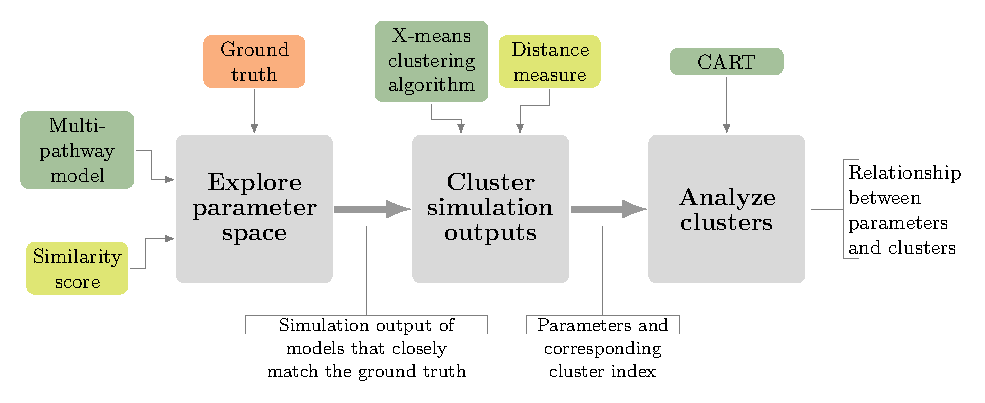
\includegraphics[width=.8\textwidth]{figs/spread_analysis.pdf}
    \caption{Outline of multi-pathway spread
analysis. \label{fig:clusterOutline}}
\end{figure}
%%
\section{Results}
%% In the first part of this section, we present results from the analysis of
%% the spread of \tuta{} in Bangladesh. We demonstrate how accounting for
%% different pathways affects the rate as well as pattern of spread. In the
%% second part, we focus on threat and possible spread in the rest of the
%% study region. The last part focuses on monitoring and control.
%%
%%
%% This section is organized as follows. We first describe the multi-pathway
%% model--our methodological contribution.  This is followed by our results in
%% the context of \tuta{} spread which are summarized as follows: (i)~We
%% identified possible routes by which \tuta{} can invade each country in the
%% region by analysis of current distribution of the pest and its.
%%
%% \paragraph{Assessing the role of each pathway in the spread of \tuta{} in
%% Bangladesh.} 
\paragraph{Variability in the pattern of spread.}
As described in Methods, the goodness of fit of a model configuration was
evaluated by comparing the corresponding simulation output with ground
truth from Bangladesh using the similarity score in~\eqref{eqn:similarity}.
Variability in the spread patterns was studied by clustering the simulation
outputs of the selected configurations (Figure~\ref{fig:clusterOutline})
and analyzing the relationship between the resulting clusters and model
parameters. The ensuing discussion will focus on instances with high
similarity score ($\similarity\ge75\%$ and approximately 8000
configurations).

For a clustering of the configuration space into two groups, the CART
analysis reveals two distinct spread patterns determined by the presence or absence of the
long-distance spread component. We observed this in the case of both
clustering algorithms. The details are in
Section~\ref{S:sec:cluster} of the supplement. We observed that even though
each of these models are a close match to the ground truth, two spread
patterns can be very different from each other. In particular, we observed
 In the first class of models
(Figure~\ref{fig:bgdClassA}) which we refer to as Class~A, the pathway
parameter~$\ald$ is negligible.  It is characterized by brisk spread
between geographically adjacent cells.  In contrast, in Class~B the
long-distance pathway~($\ald$) plays a significant role
(Figure~\ref{fig:bgdClassB1}) and is characterized by relatively slow
spread between geographically adjacent neighbors with jumps from one
locality to another.

%% %% It is characterized by %%
%% a combination of Moore range ($\mooreRange$), latency period ($\ell$) and
%% %% pathway parameters~$\asd$ and~$\afm$ that lead to rapid spread between
%% %% adjacent cells.  
%%
\begin{figure}[!ht]
    \centering
\begin{subfigure}[b]{.4\textwidth}
    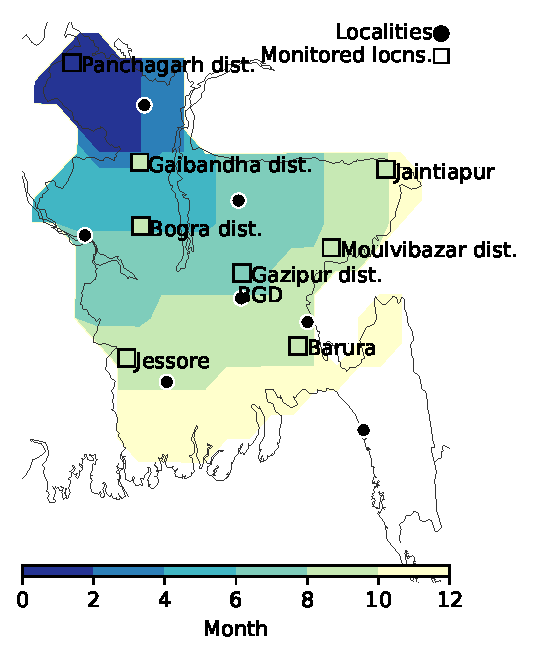
\includegraphics[width=\textwidth]{../cellular_automata/results/contour/BGD_model-A.pdf}
    \caption{Class~A ($\ald=0$) \label{fig:bgdClassA}}
\end{subfigure}\hspace{.5cm}
\begin{subfigure}[b]{.4\textwidth}
    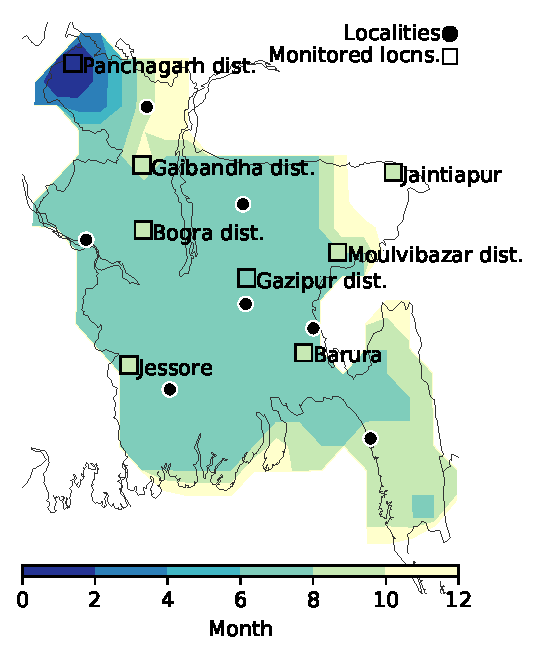
\includegraphics[width=\textwidth]{../cellular_automata/results/contour/BGD_model-B_m1_l3.pdf}
    \caption{Class~B ($\ald>0$) \label{fig:bgdClassB1}}
\end{subfigure}
\caption{\textbf{Spread in Bangladesh.}The contour plots show the simulated
spread starting from the location of first report in Panchagarh district
for 12 months. For the purpose of plotting, the time of infection for a
cell is the minimum time step~$t$ such that the empirical probability that
the cell is infected by time~$t$ is $\ge0.8$. Also highlighted are the
eight monitored locations and the localities applied in the model. The
colors of the monitored locations correspond to the month of report
relative to the first report (Panchagarh). Two distinct spread patterns
emerged from the cluster analysis. (a) and (b) show representative spreads
observed for each class. The similarity ($\similarity$) in each case was
$>6.5$.}
%% (a)~\textbf{Class~A.} Spread pattern long-distance component playing a
%% negligible role. We
%% observe a steady radial spread.  (b)~\textbf{Class~B.} Spread pattern with
%% long-distance jumps. Here, the radial spread is much slower.}
\end{figure}
%%
Class~A spread pattern does not capture the gap between the time of first
report (Panchagarh) and the report in Gaibandha district
(Figure~\ref{fig:bgdClassA}). Even though the distance between the two
locations is only $185$kms, the latter reported the presence only after~10
months of first report suggesting that self-mediated spread might have been
much slower. In the model output on the other hand, the corresponding cell
gets infected between the second and fourth months.  In Class~B, this
location is infected much later in comparison. However, the eastward spread
towards the location Jaintiapur is slower than what was observed
(Figure~\ref{fig:bgdClassB1}). Even though Panchagarh is quite far from
this location, pest presence was reported by February 2017, just nine
months from the first report.  

We also simulated the spread using the cellular automata model developed by
Guimapi~\cite{guimapi2016modeling} for Bangladesh. The spread pattern is
similar to Class~A as the model does not account for long-distance
hops. However, the predicted rate of range expansion is much higher than
our models (see Section~\ref{S:sec:guimapi} for model details and results).


\paragraph{Importance of model parameters.} 
Calibration and sensitivity analysis of large-scale, high-resolution models
is a challenging task. Methods based on machine learning surrogates are
being increasingly used to accomplish this efficiently for complex
agent-based models~\cite{lamperti2018agent}. We studied sensitivity of the
spread pattern to model parameters by applying Random Forest learning
method. Since the clustering captures the variations in spread patterns,
the algorithm was applied with model parameters as independent variables
and cluster index as the dependent variable. The results are in
Figure~\ref{fig:sensitivity}.
%%
%% \begin{figure}[t]
%% \centering
%% \begin{subfigure}[b]{.32\textwidth}
%%     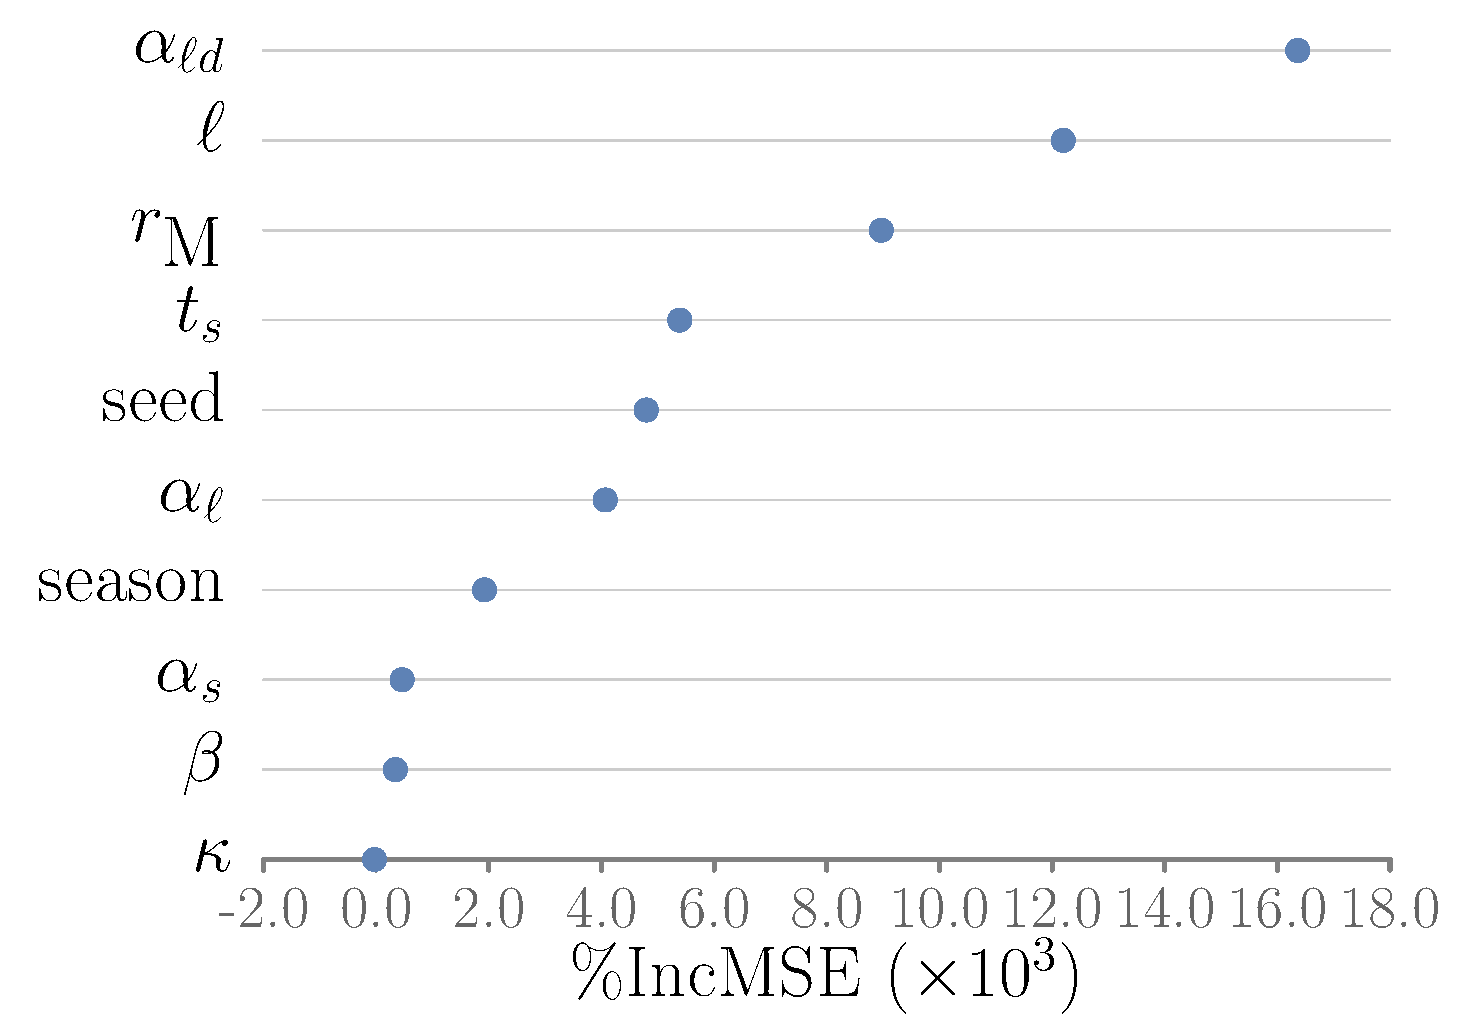
\includegraphics[width=1.1\textwidth]{../clustering/results/rf_importance_cluster_mse_all.pdf}
%%     \caption{All \label{fig:rfAll}}
%% \end{subfigure}
%% %%
%% \begin{subfigure}[b]{.32\textwidth}
%%     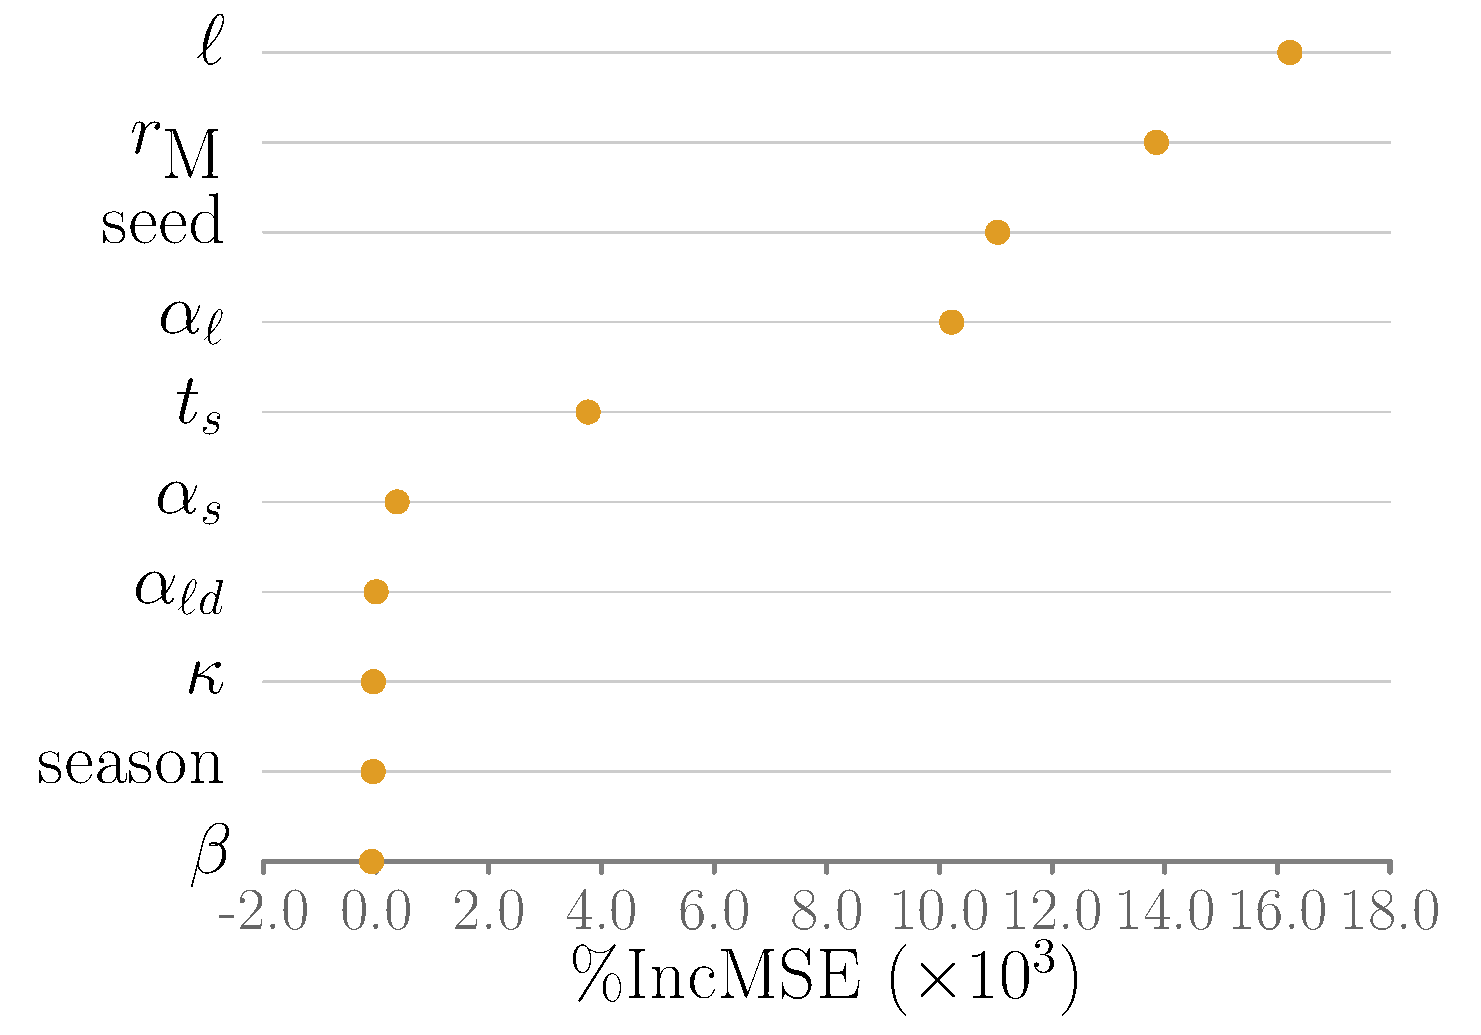
\includegraphics[width=1.1\textwidth]{../clustering/results/rf_importance_cluster_mse_A.pdf}
%%     \caption{Class A\label{fig:rfA}}
%% \end{subfigure}
%% %%
%% \begin{subfigure}[b]{.32\textwidth}
%%     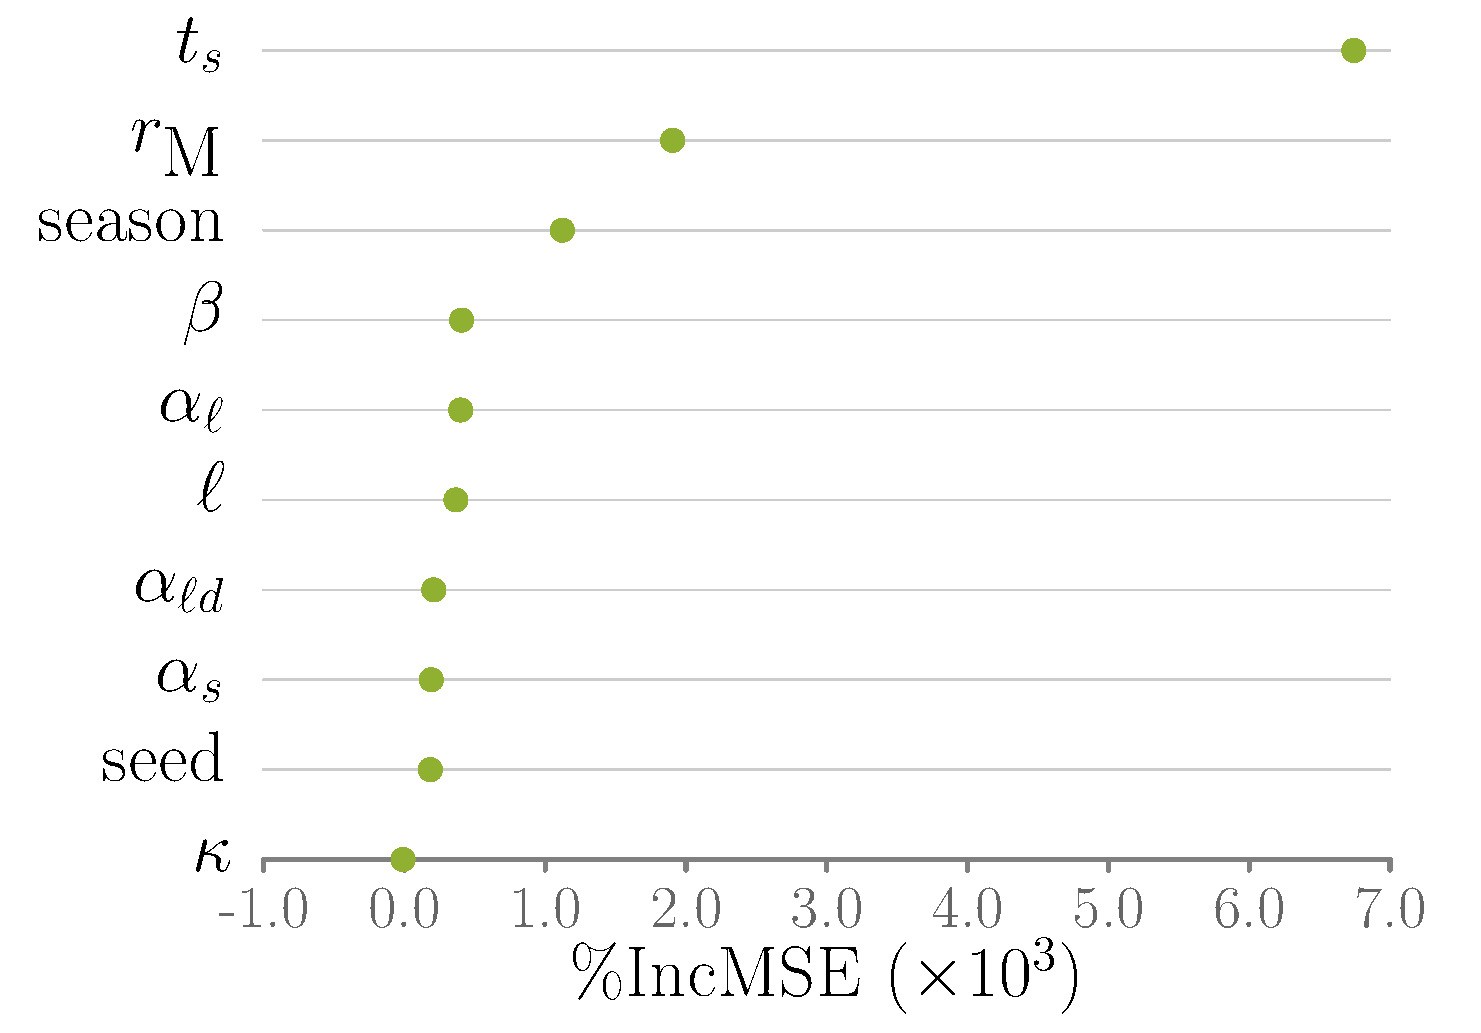
\includegraphics[width=1.1\textwidth]{../clustering/results/rf_importance_cluster_mse_B.pdf}
%%     \caption{Class B\label{fig:rfB}}
%% \end{subfigure}
%% %%
%% \begin{subfigure}[b]{.32\textwidth}
%%     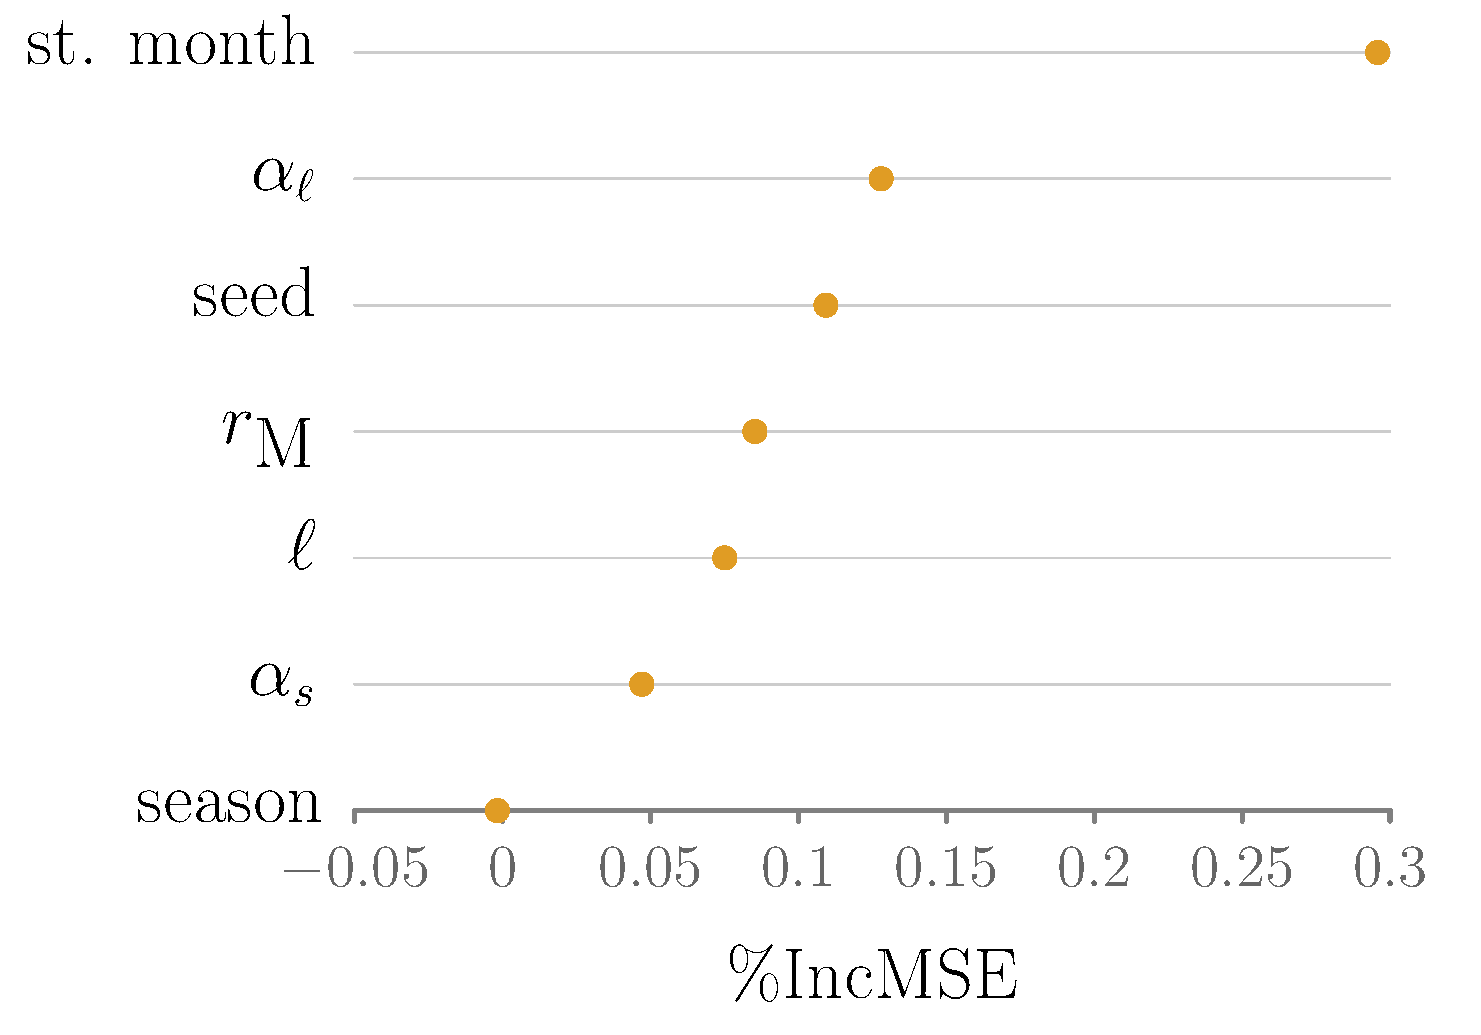
\includegraphics[width=1.1\textwidth]{../cellular_automata/results/rf/rf_importance_short_mse.pdf}
%% \caption{Class A\label{fig:rfShort}}
%% \end{subfigure}
%% %%
%% \begin{subfigure}[b]{.32\textwidth}
%% 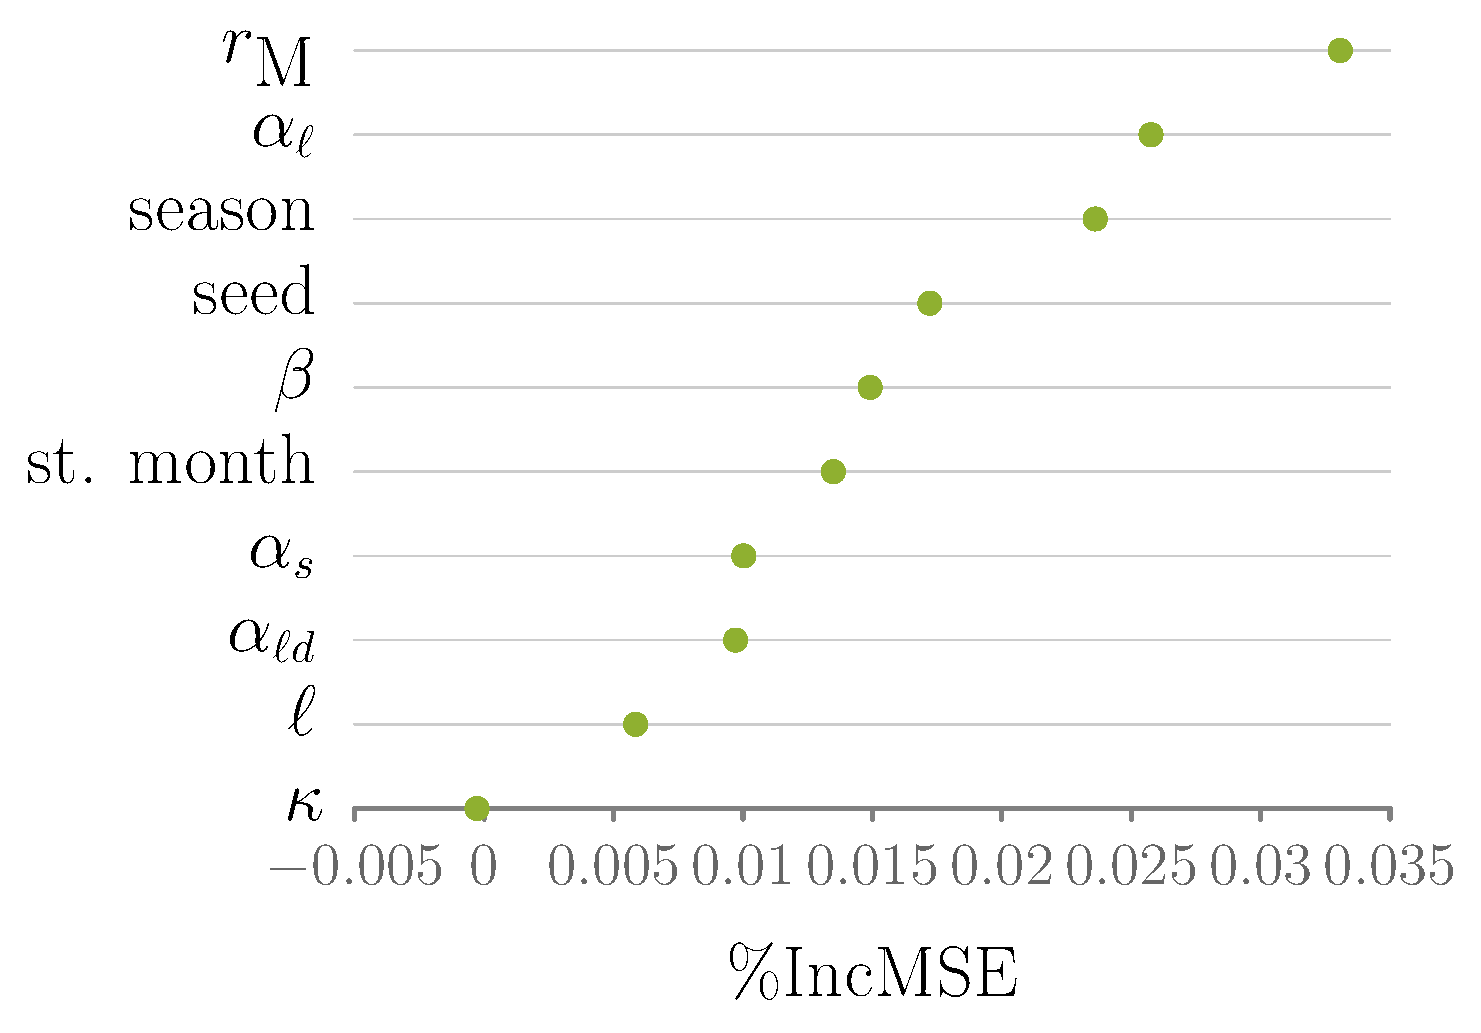
\includegraphics[width=1.1\textwidth]{../cellular_automata/results/rf/rf_importance_long_mse.pdf}
%% \caption{Class B\label{fig:rfLong}}
%% \end{subfigure}
%%\caption{\textbf{Parameter importance.} Random
%%Forest~\cite{breiman2001random} method was applied to study parameter
%%importance. (a)~With cluster index as the dependent variable,
%%the analysis was performed on the set of model instances which yielded a
%%similarity~$\similarity\ge6$.
%%%% (b)~The sensitivity of the spread pattern to parameters was analyzed by
%%%% repeating the same process, but with cluster index as the dependent
%%%% variable.
%%The results for the entire set (a) and separately for Class~A (b) and
%%Class~B models (c) are shown. The parameters are ordered by their
%%importance based on percentage increase in mean square error from permuting
%%the variable--higher, the more important.
%%\label{fig:sensitivity}}
%%%% a total of $17,000$ samples from the parameter space
%%\end{figure}
%%

The long distance pathway parameter~$\ald$ is by far the most important
parameter (Figure~\ref{fig:rfAll}); both spread rate and pattern critically
depend on it. Moore range ($\mooreRange$) and latency period ($\ell$) are
important as they affect the rate of radial spread. The start month ($t_s$)
is also important due to two reasons. Firstly, the distance between two
time shifted simulation outputs can be large. Secondly, outputs are
sensitive to seasonal variations or temporality of the network. Focussing
on Class~A models, the main drivers of the spread pattern are latency
period and Moore range (Figure~\ref{fig:rfA}). Since the simulation
duration represents more than one year of spread, seasonality (season) does
not have much effect on the spread. The distance parameters~$\beta$
and~$\kappa$ do not influece the spread as~$\ald=0$. Seasonal production on
the other hand is very important in Class~B models as it influences trade
flows.

Class~B models show more sensitivity to start time step of simulation than
Class~B models. The main reason why it is not at all critical in the latter
class is because the pest was reported just before the rainy season;
subsequent months have lean trade flows, and as a result it does not affect
the spread much. However, it does not seem to have much effect on the
radial spread component as is the case with Class~A models. In both cases,
the spread is very sensitive to the local human-mediated pathway
parameter~$\afm$. In the case of Class~A models, this pathway leads to
faster spread within localities. In Class~B models, higher the value, the
greater the chance of long-distance spread as it quickly leads to infection
of large portions of the localities, and therefore their total
infectiousness. Later, we will discuss on how it influences the spread rate
for the rest of the region.
%% \begin{figure}[ht]
%%     \centering
%%     \begin{subfigure}[b]{.48\textwidth}
%% 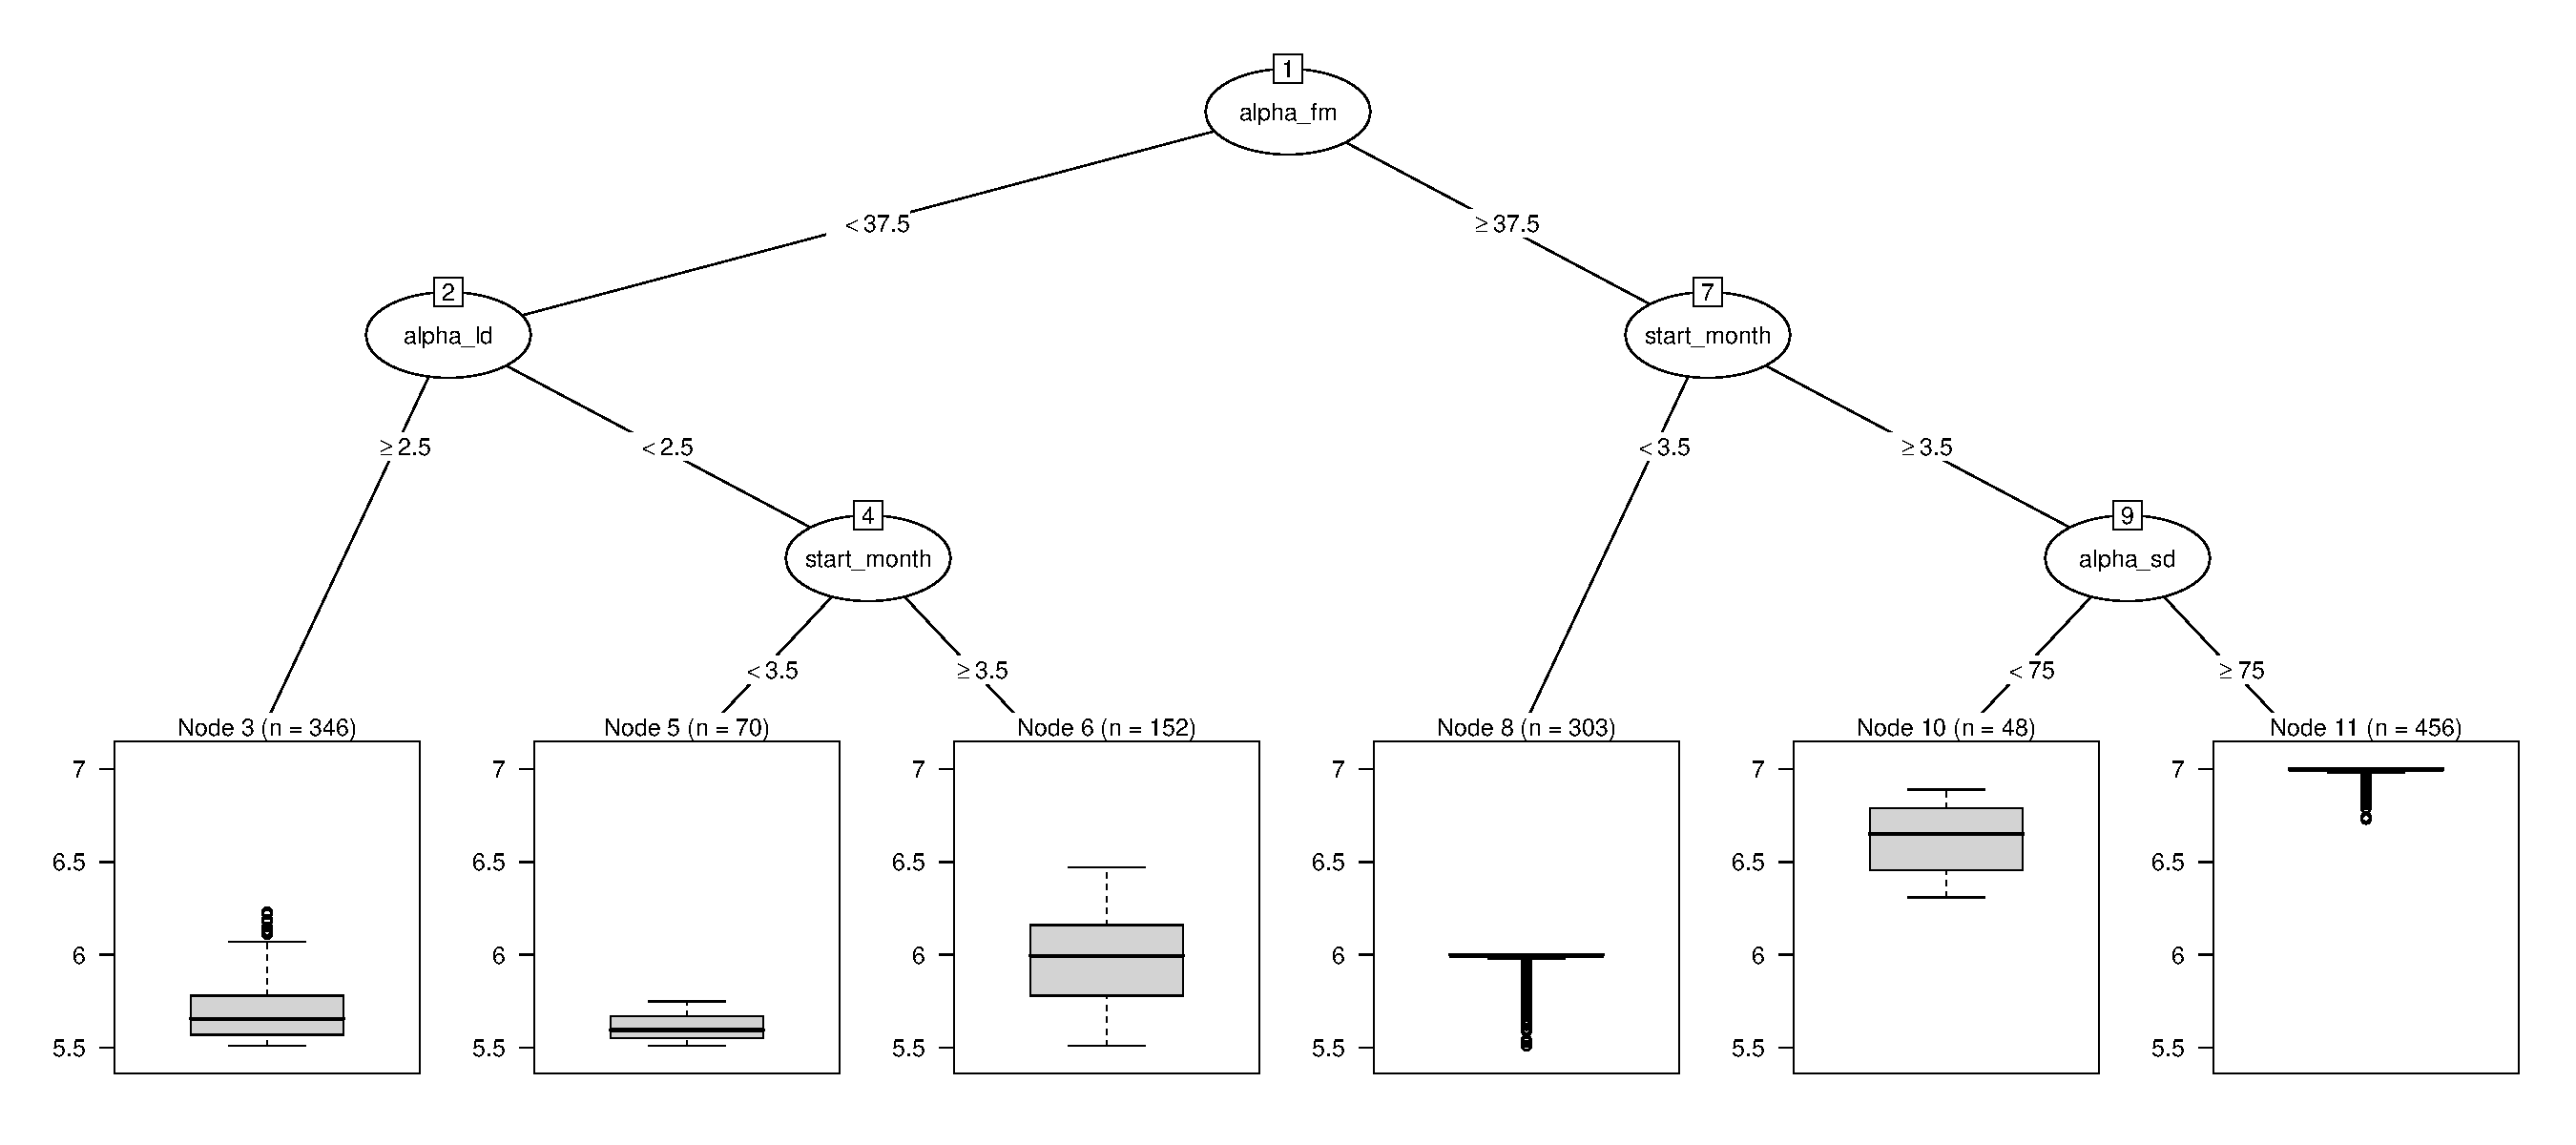
\includegraphics[width=\textwidth,trim={1cm 1cm 1cm 1cm},clip]{../cellular_automata/results/cart/m2_l2_tree.pdf}
%%     \caption{$\mooreRange=2$, $\ell=2$ \label{fig:cart22}}
%%     \end{subfigure}
%%     \begin{subfigure}[b]{.48\textwidth}
%% 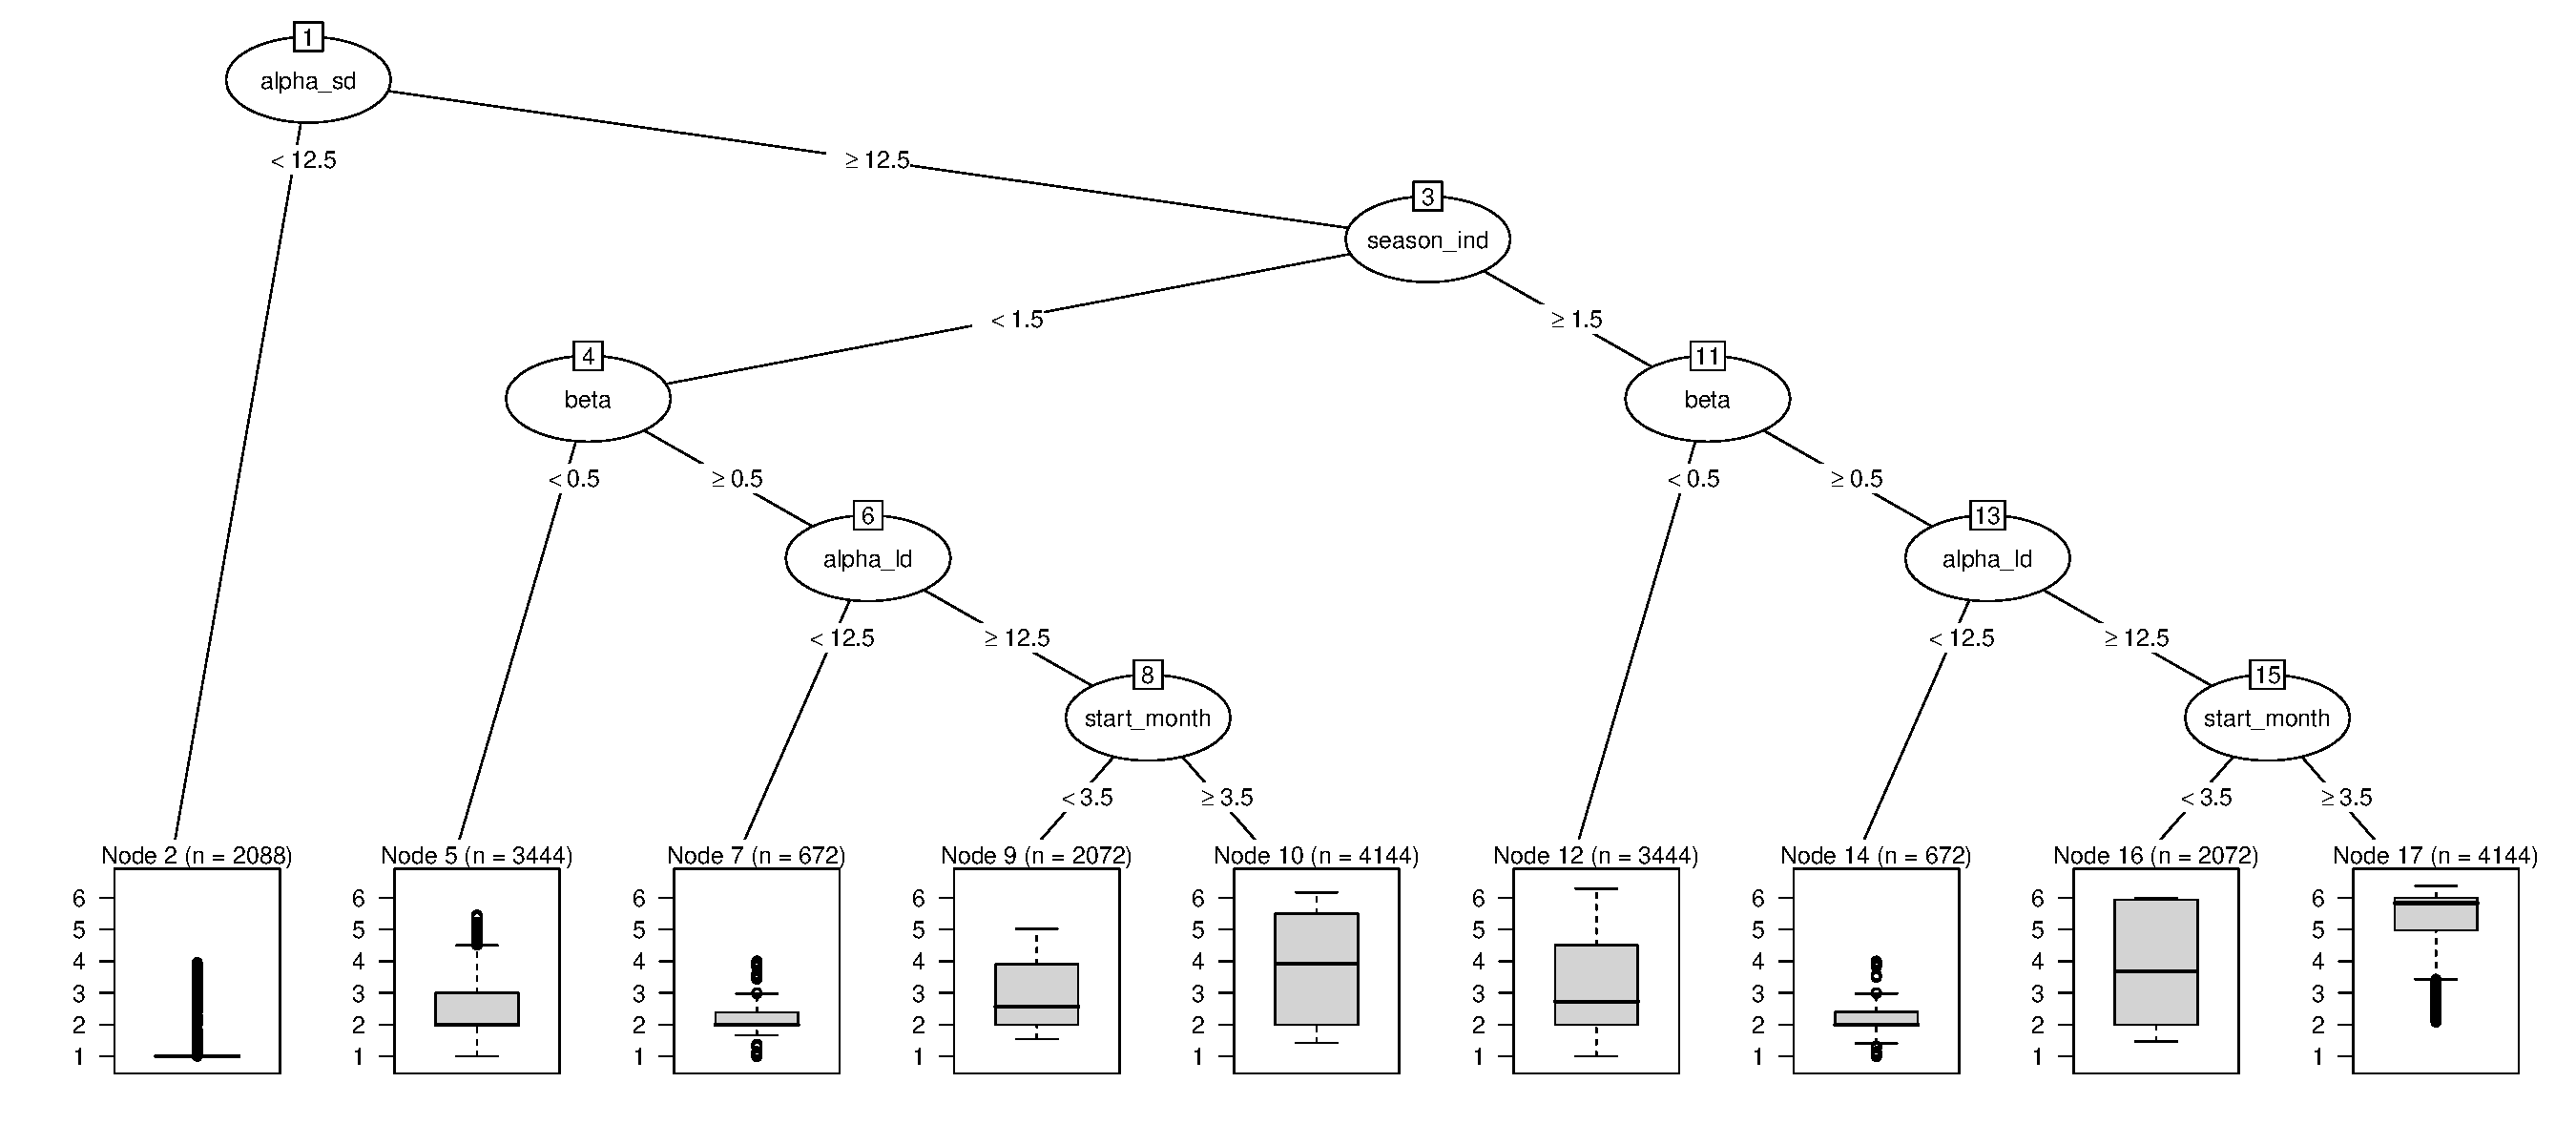
\includegraphics[width=\textwidth,trim={1cm 1cm 1cm 0cm},clip]{../cellular_automata/results/cart/m2_l3_tree.pdf}
%%     \caption{$\mooreRange=2$, $\ell=3$ \label{fig:cart32}}
%%     \end{subfigure}
%%     %% \begin{subfigure}[b]{.48\textwidth}
%%     %% 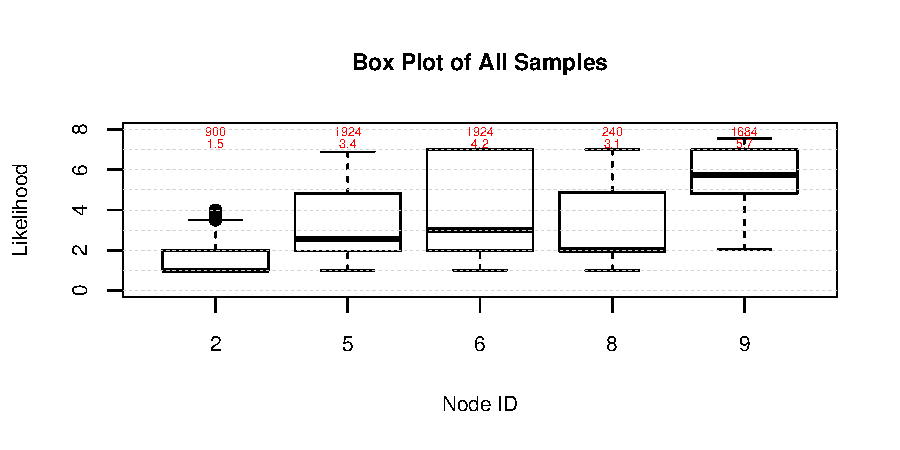
\includegraphics[width=\textwidth]{figs/cart_box1.pdf}
%%     %% \caption{\label{fig:cartBox1}}
%%     %% \end{subfigure}
%%     %% \begin{subfigure}[b]{.48\textwidth}
%%     %% 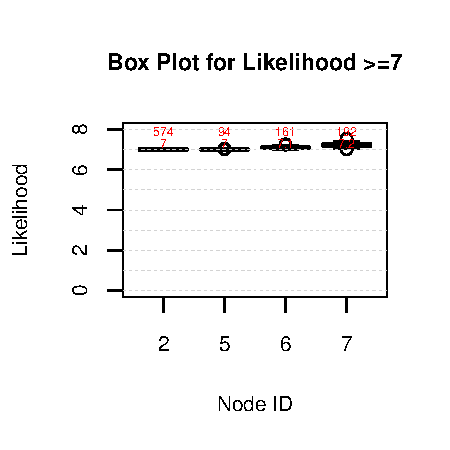
\includegraphics[width=\textwidth]{figs/cart_box2.pdf}
%%     %% \caption{\label{fig:cartBox2}}
%%     %% \end{subfigure}
%%     \caption{CART analysis of the parameter space: The models with
%%         similarity$\ge5.5$ were partitioned based on the Moore
%%     range~$\mooreRange$ and latency period~$\ell$ tuple and analyzed. Two
%%     of the nine cases are shown. The complete set is in
%%     Figure~\ref{S:fig:cart}.}
%% \end{figure}
%%
\paragraph{Domestic trade and spread within a country.}
Here, we focus on long-distance dispersal, and therefore, restrict our
discussion to Class~B models. We observed the following common spread
pattern.  When the pest is introduced to a country, dispersal is slow until
the invasion front reaches a locality close to a \emph{source}, one with
significant outflows to other localities. Once it establishes at a source,
the spread is very fast and within a year or two, it spreads to almost all
major localities of the country. There is a possibility that \tuta{} can be
introduced to a country several months before it becomes pervasive. 
%% Our
%% results show that for all countries, once the pest is introduced, within
%% 2-3 years the it will spread to almost all localities, and when it reaches
%% a high production locality, it spreads to other regions within a year.
%% Past invasion records support this trend.
%% The pest became widespread in
%% countries Mediterranean
%% region, in Middleeastern countries, and in India in just 2-3 years.

We recall the discussion about the slow spread rate of our models in
Mainland Southeast Asia compared to the spread in Bangladesh. In the case
of Class~B models, another
reason for the reduced spread rate could be due to ignoring some trade
flows between countries. Because of
this, we observe a slow spread at the country boundaries.
Historically, international trade has played a strong role in the spread of
\tuta{} between countries in Europe
and West Asia.  This seems to apply to even South Asia. The pest was first
reported by India
in~2014~\cite{sridhar2014new,kalleshwaraswamy2015occurrence}. By
early~2016, it was discovered in the Kathmandu area of
Nepal~\cite{bajracharya2016first}, the northern part of Bangladesh in
May~2016~\cite{hossain2016first}. Both countries import significant volume
of tomato from India. However, there has been no report from Pakistan,
another neighbor which does not import tomato from India. It is possible
that the pest is present and undetected in this country. But, it is clear
that Pakistan is aware of the threat\footnote{The looming threat of the
deadly tomato leafminer~(\url{https://www.dawn.com/news/1420206}).} indicating that even
if it is present, it is not widespread. There are similar examples outside the
region such as its slow advance from South America to Central America, or
the fact that it is not reported in China despite being present in
neighboring Central Asian countries since~2015. Hence, it is critical to
address the data gaps concerning international trade.

%% However, we recall that trade between some countries was ignored, and as a
%% result our model might have missed some long-distance jumps.  For example,
%% from Vietnam, there is a possibility that it can enter Phnom Penh, Cambodia
%% through tomato imports during the rainy months~\cite{sokhen2004}. The
%% southwards spread to Malaysia might be faster than predicted by Class~B
%% spread due to exports from Thailand to Malaysia and Singapore.
%%
%% We used both model classes to study the spread in the rest of the
%% region. We applied them to the region as a whole as well as each
%% country separately. For the whole region, the starting point of the
%% spread corresponds to cell~(a) (Figure~\ref{fig:bgdRadial}). For the
%% country-specific studies, the starting location was decided based on
%% our analysis of possible entry points through natural spread as well as
%% trade. The results are in Figures~\ref{fig:totalSpread}
%% and~\ref{fig:spreadWithin}. Both
%% cases strongly indicate that \tuta{} is present in parts of Myanmar
%% (curves corresponding to timestep 24 or two years from first report).
%% Class~A predicts that the entire Mainland Southeast Asia will be infested
%% with four years.
%% %% We considered three scenarios of introduction of the pest to the region.
%% %% The first scenario corresponds to evolution of the spread from Bangladesh
%% %% (B1). The other two are hypothetical scenarios based on the analysis in
%% %% Section~\ref{sec:entry}. Scenario~M corresponds to \tuta{} introduced near
%% %% a major port region of Malaysia. The third Scenario~P is its introduction
%% %% to Philippines close to the captial city Manila assuming introduction
%% %% due to migratory workers from \tuta{} affected regions.
%% 
%% From Figure~\ref{fig:totalSpread}, we observe that the range expansion is
%% much faster with Class~A compared to Class~B. The main reason for the slow
%% spread is due to not accounting for trade interactions between countries in
%% the model. The spread is characterized by slow spread between countries and
%% rapid expansion within. For example, the big jumps in range expansion
%% between time steps 72 and 120 is mainly due to spread within Myanmar
%% through long-distance jumps. The challenges in modeling international trade
%% are covered in Methods (Trade flows). But when we consider the global
%% spread pattern of \tuta{}, we observe reduction in rate of range expansion
%% in certain regions.
%% 
%% Also, the predicted spread could be
%% slower due boundary effects; we have not accounted for cells belonging to
%% Northeastern parts of India that share border with Bangladesh and Myanmar
%% and the Yunnan province of China.  On the other hand, when we focus on each
%% country separately (Figure~\ref{fig:spreadWithin}, we observe that the
%% spread within a country is much faster in the case of Class~B.  Results
%% suggest that major production areas of a country will be invaded within 2-3
%% years of introduction.
%% 
%% The spatio-temporal spread for Scenario~B1 is shown in
%% Figure~\ref{fig:spreadBGD}. The start time corresponds to~24 time steps (or
%% two years) from the first report. The results indicate that there is a high
%% chance that \tuta{} will spread to Mainland Southeast Asia in four to six
%% years. Because of long distance dispersal, we also observe a non-radial
%% spread. Aided by domestic trade and exports from Thailand, there is
%% possibility that the pest will be introduced to Peninsular Malaysia and
%% subsequently to Singapore and Indonesia in this period even though this
%% area is much farther from the current range of \tuta{}. Also, we see the
%% possibility of the pest crossing the sea from Peninsular Malaysia to
%% Malaysian Borneo within a year of introduction to this country. However,
%% these are conservative estimates. First of all, the simulations do not
%% account for possible new introductions. 

%% The spread due to other two scenarios are shown in Figures~\ref{spreadMYS}
%% and~\ref{spreadPHL} respectively. Note that in both of these scenarios we do not
%% account for the spread from Bangladesh. This is crucially dependent on the
%% time of introduction. However, it is critical to consider the synergistic
%% effects of range expansion from multiple locations. The spread in
%% Scenario~M follows a similar pattern as in Scenario~B3.
%% \aacomment{Philippines pending}.

%% \begin{figure}[ht]
%%     \centering
%%     \begin{subfigure}[b]{.32\textwidth}
%%         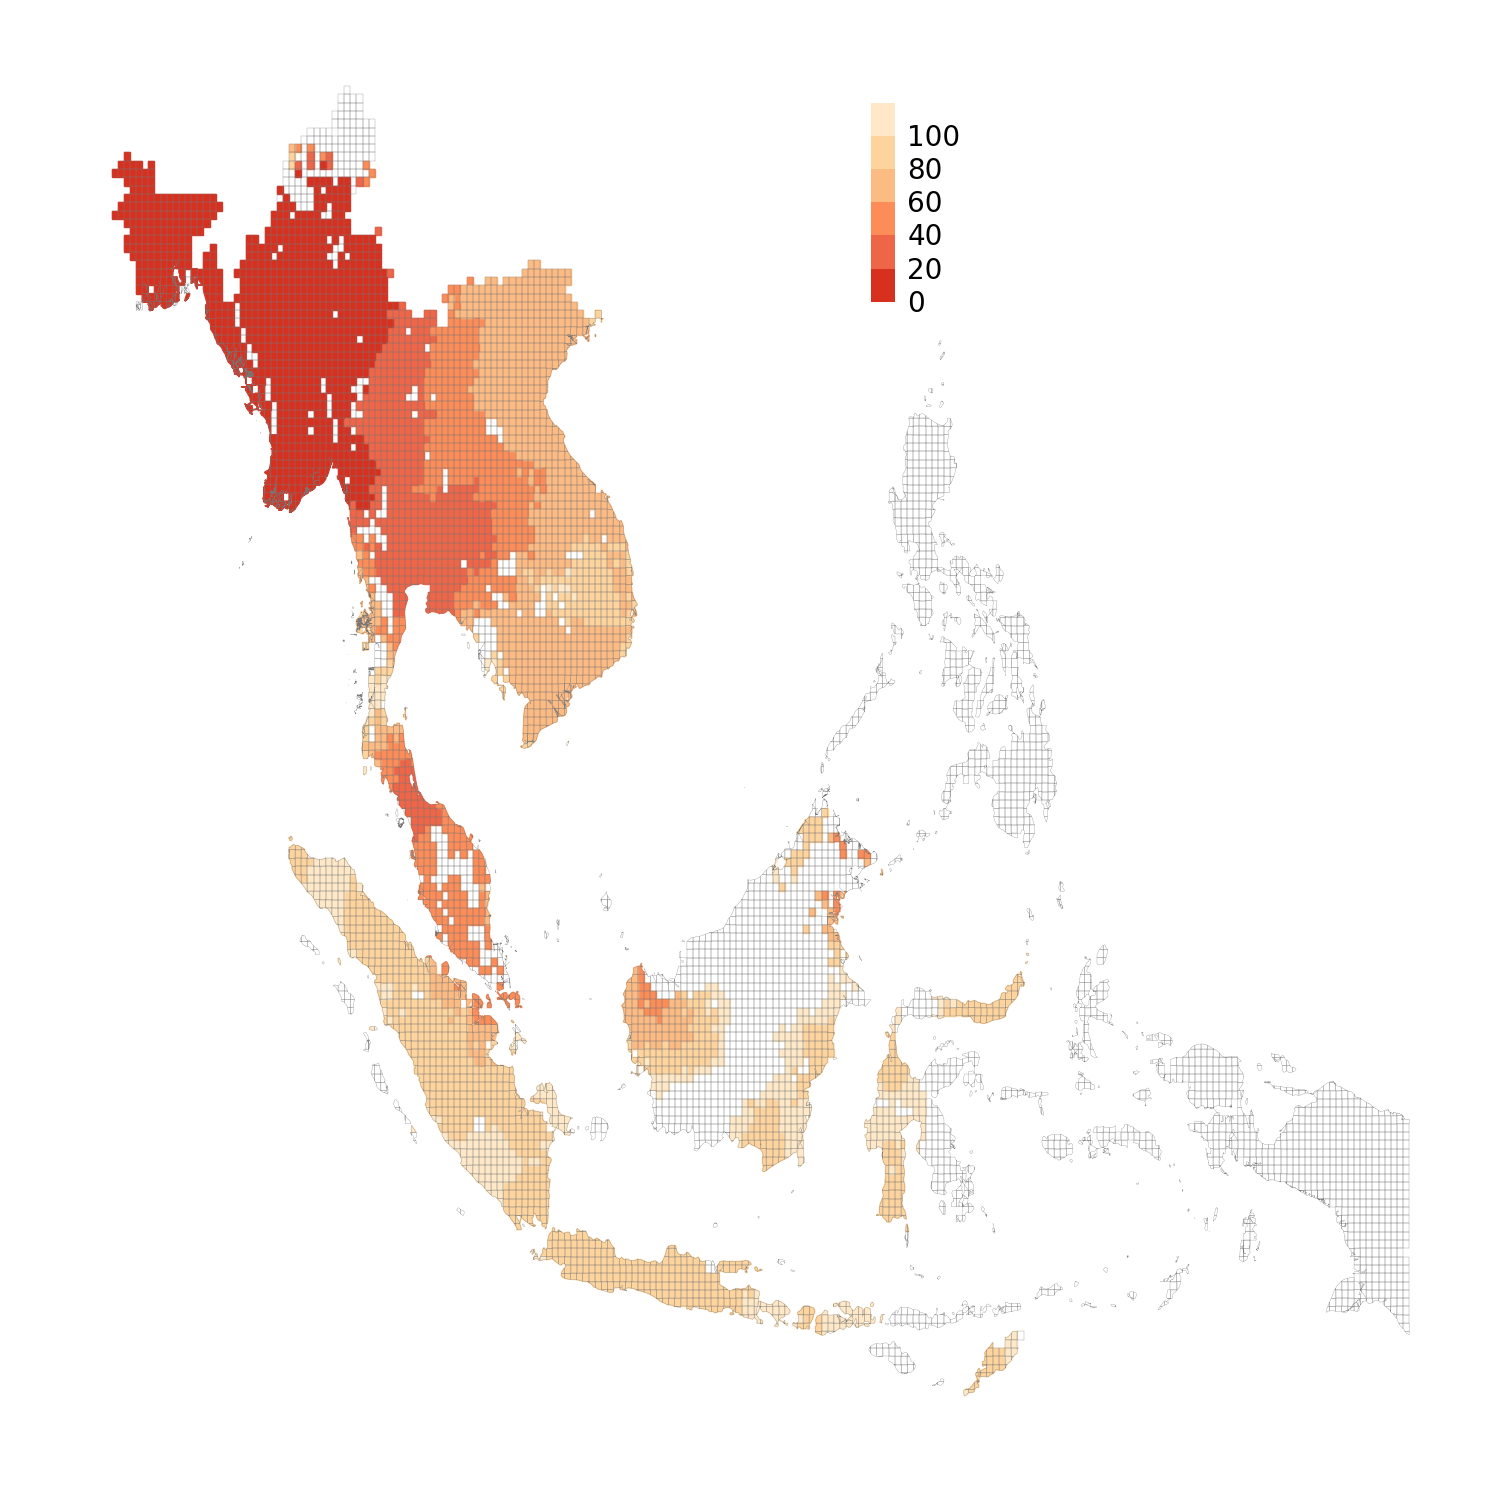
\includegraphics[width=\textwidth,trim={3cm 3cm 8cm 3cm},clip]{figs/spread_BGD.png}
%%     \caption{Scenario~B1\label{fig:spreadBGD}}
%%     \end{subfigure}
%%     \begin{subfigure}[b]{.32\textwidth}
%%         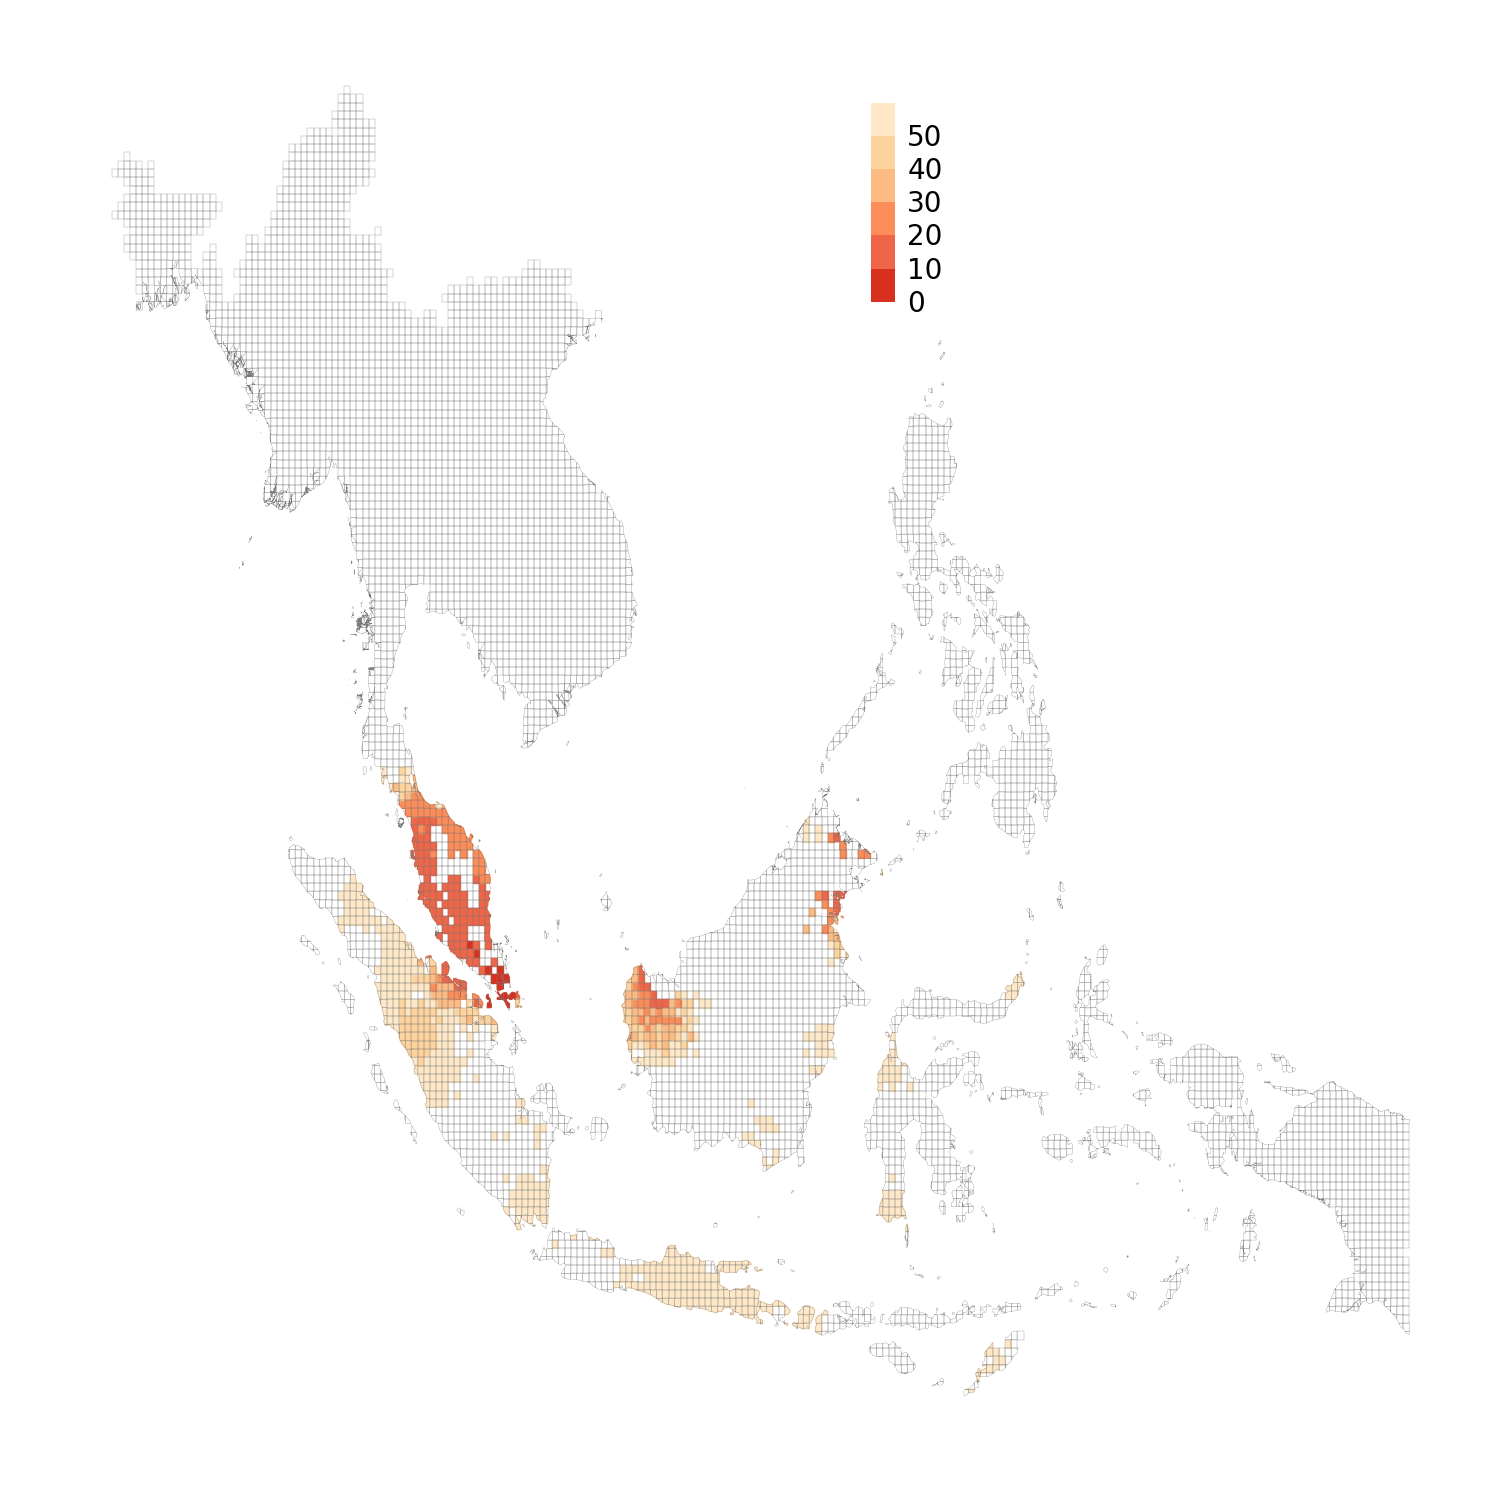
\includegraphics[width=\textwidth,trim={4cm 2cm 8cm 12cm},clip]{figs/spread_MYS.png}
%%     \caption{Scenario~M\label{fig:spreadMYS}}
%%     \end{subfigure}
%%     \begin{subfigure}[b]{.32\textwidth}
%%         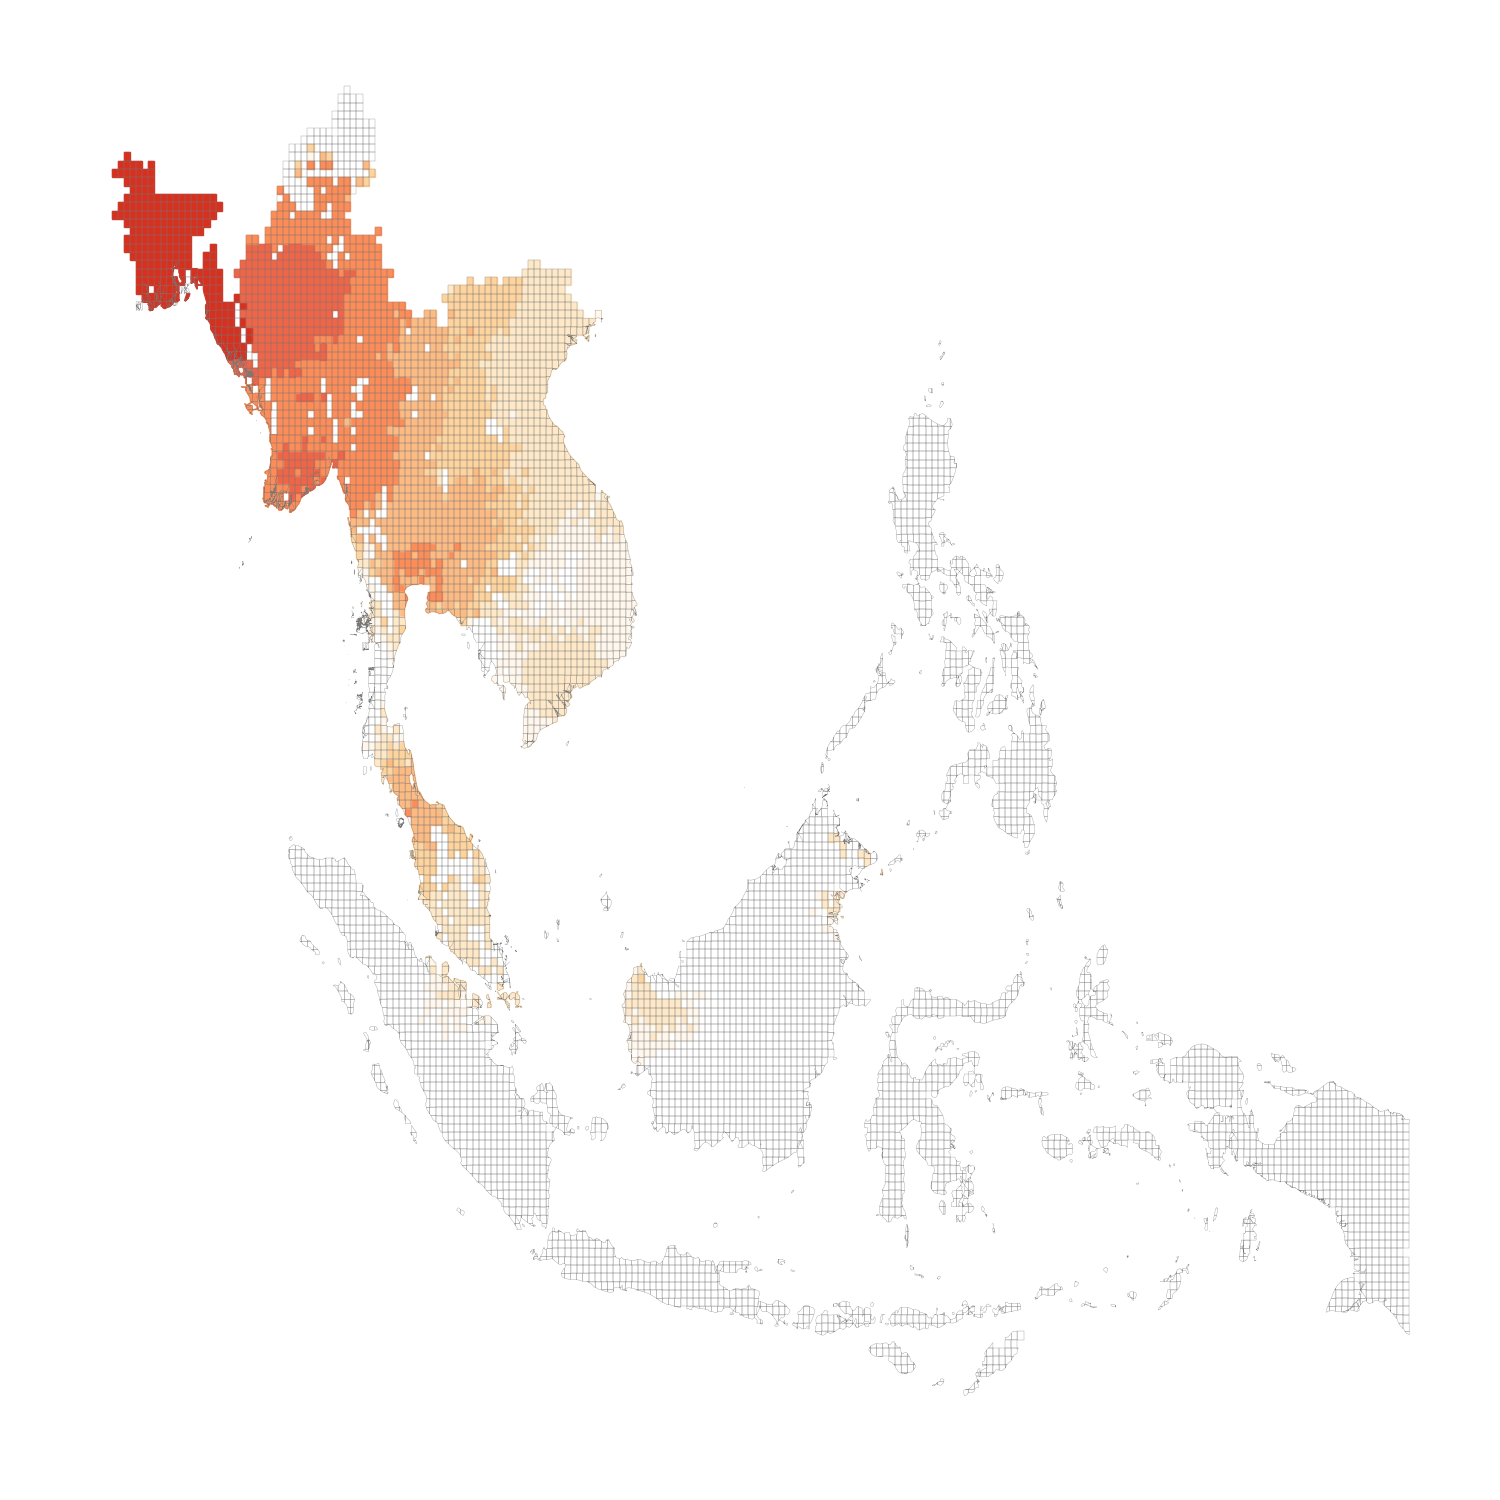
\includegraphics[width=\textwidth,trim={4cm 2cm 8cm 12cm},clip]{figs/spread_PHL.png}
%%     \caption{Scenario~P\label{fig:spreadPHL}}
%%     \end{subfigure}
%%     \caption{Possible spread of \tuta{} in the focus region under three
%%     scenarios. In each plot, the legends correspond to months. For the
%%     purpose of plotting, for each cell, we compute the time~$t$ for which
%%     the empirical probability of infection before~$t$ is at least $0.1$.
%%     Scenario~B3 starts with Bangladesh and significant parts of Myanmar
%%     infested accounting for spread from May 2016 to May 2018.
%%     \aacomment{Philippines pending, legend will be made bigger}}
%% \end{figure}

%%
%% Specific observations
%% \begin{itemize}
%%     \item identify important vegetable production areas
%% \end{itemize}

%%
%% Among the countries listed in the FAOSTAT dataset, Indonesia is by far the
%% largest producer ($\approx1$M tonnes) followed by Philippines and Malaysia
%% ($\approx200$K tonnes each). However, alternate data sources (pers.
%% comm.) indicate that Vietnam is a large producer ($\approx400$K)
%% too.
%%
%% \paragraph{Predicted spread in Mainland Southeast Asia.}
%% We applied both model classes to simulate the spread in the rest of the
%% study region. Given that more than two years have passed since the time of
%% first report in Bangladesh and unofficial reports of \tuta{} presence in
%% Myanmar\footnote{The Wikipedia entry on \tuta{}
%%     (\url{https://en.wikipedia.org/wiki/Tuta_absoluta}) indicates
%% that it is present in the northern region of Myanmar since
%% April~2017. No official confirmation is available yet.}, cells in northern Myanmar bordering India and Bangladesh were
%% seeded (Methods). Representative simulation outputs are shown for Mainland
%% Southeast Asia in Figure~\ref{fig:msaClassAB}. We note that in the case of
%% Class~A models, the eastward spread is faster than southward spread. This
%% is mainly because the Moore neighborhood is smaller at the narrow region in
%% the south of Myanmar and Thailand bordering Malaysia. However, in
%% the case of Class~B, the spread is much faster in the same region aided by domestic
%% trade flows from northern and central Thailand to the southern region. Both models indicate that the pest will enter
%% Thailand from Myanmar, and subsequently move to Laos and Vietnam as it
%% spreads eastwards and to China when it spreads northwards.
%% %%
%% %Changed B to A
%% \begin{figure}[ht]
%%     \centering
%% \begin{subfigure}[b]{.47\textwidth}
%%     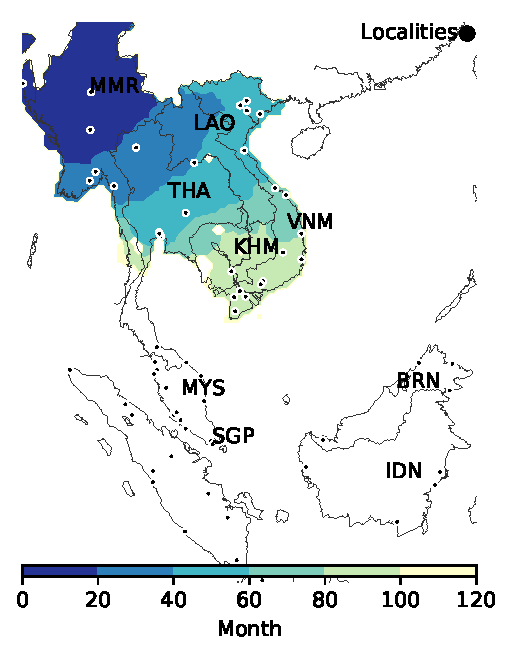
\includegraphics[width=\textwidth]{../cellular_automata/results/contour/MSA_model-A_m2_l1.pdf}
%%     \caption{Class~A\label{fig:msaClassA}}
%% \end{subfigure}\hspace{.5cm}
%% \begin{subfigure}[b]{.47\textwidth}
%%     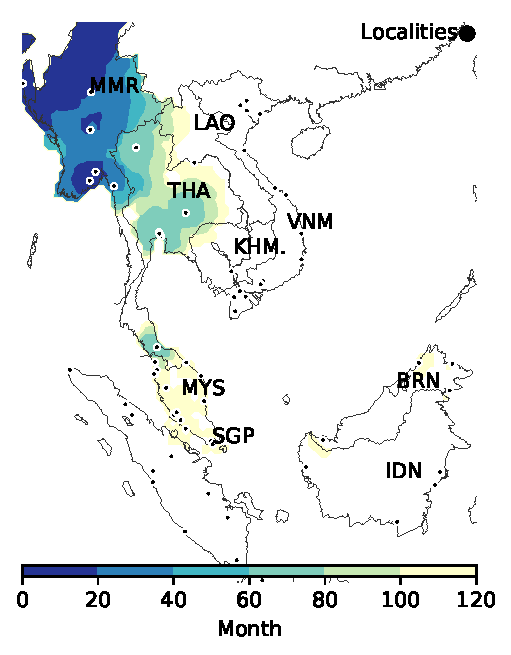
\includegraphics[width=\textwidth]{../cellular_automata/results/contour/MSA_model-B_m1_l3.pdf}
%%     \caption{Class~B\label{fig:msaClassB}}
%% \end{subfigure}
%% \caption{\textbf{Predicted spread pattern in Mainland Southeast Asia.} The
%% contour plots show the simulated spread starting from northern Myanmar for
%% 120 time steps or 10 years. Representative simulation outputs for Class~A
%% and Class~B models are shown. With {Class~A}, spread is faster eastward
%% than southward and the other way round in the case of
%% Class~B.\label{fig:msaClassAB} }
%% \end{figure}
%% %%
%% 
%% Class~A spread pattern predicts that within the next 4-5 years much of the
%% northern part of Mainland Southeast Asia will be invaded. Class~B spread
%% pattern predicts that in the same period \tuta{} will spread all over
%% Malaysia and Singapore.  However, the rate of spread observed is slower
%% than that observed in Bangladesh for both classes. Also, even though the
%% models exhibited similar rate of spread for Bangladesh, we observed high
%% variance in intensity of infestation as well range expansion for the rest
%% of the region. The results are in Figure~\ref{fig:spreadRate}. The reason
%% for slow spread is as follows.  Bangladesh has the highest tomato volume
%% per country surface area ($\approx2.5$tonnes/km$^2$).  The next country is
%% Vietnam ($\approx1.5$tonnes/km$^2$). Therefore, in the case of Bangladesh,
%% not only is the extent of infestation in a cell~$\infest(\cdot)$ typically
%% high, but also, since it is a densely populated country, most cells have
%% vegetable production. Hence, the rate of spread is much higher for
%% relatively lower values of pathway parameters and Moore range. Also, we
%% observed a strong dependence on Moore range (Figure~\ref{fig:spreadRateB}).
%% In countries with larger area, the production is scattered. Therefore,
%% lower the Moore range, the slower the spread.
%% %%   
%% \begin{figure}[!ht]
%% %% \begin{subfigure}[b]{.47\textwidth}
%% %%     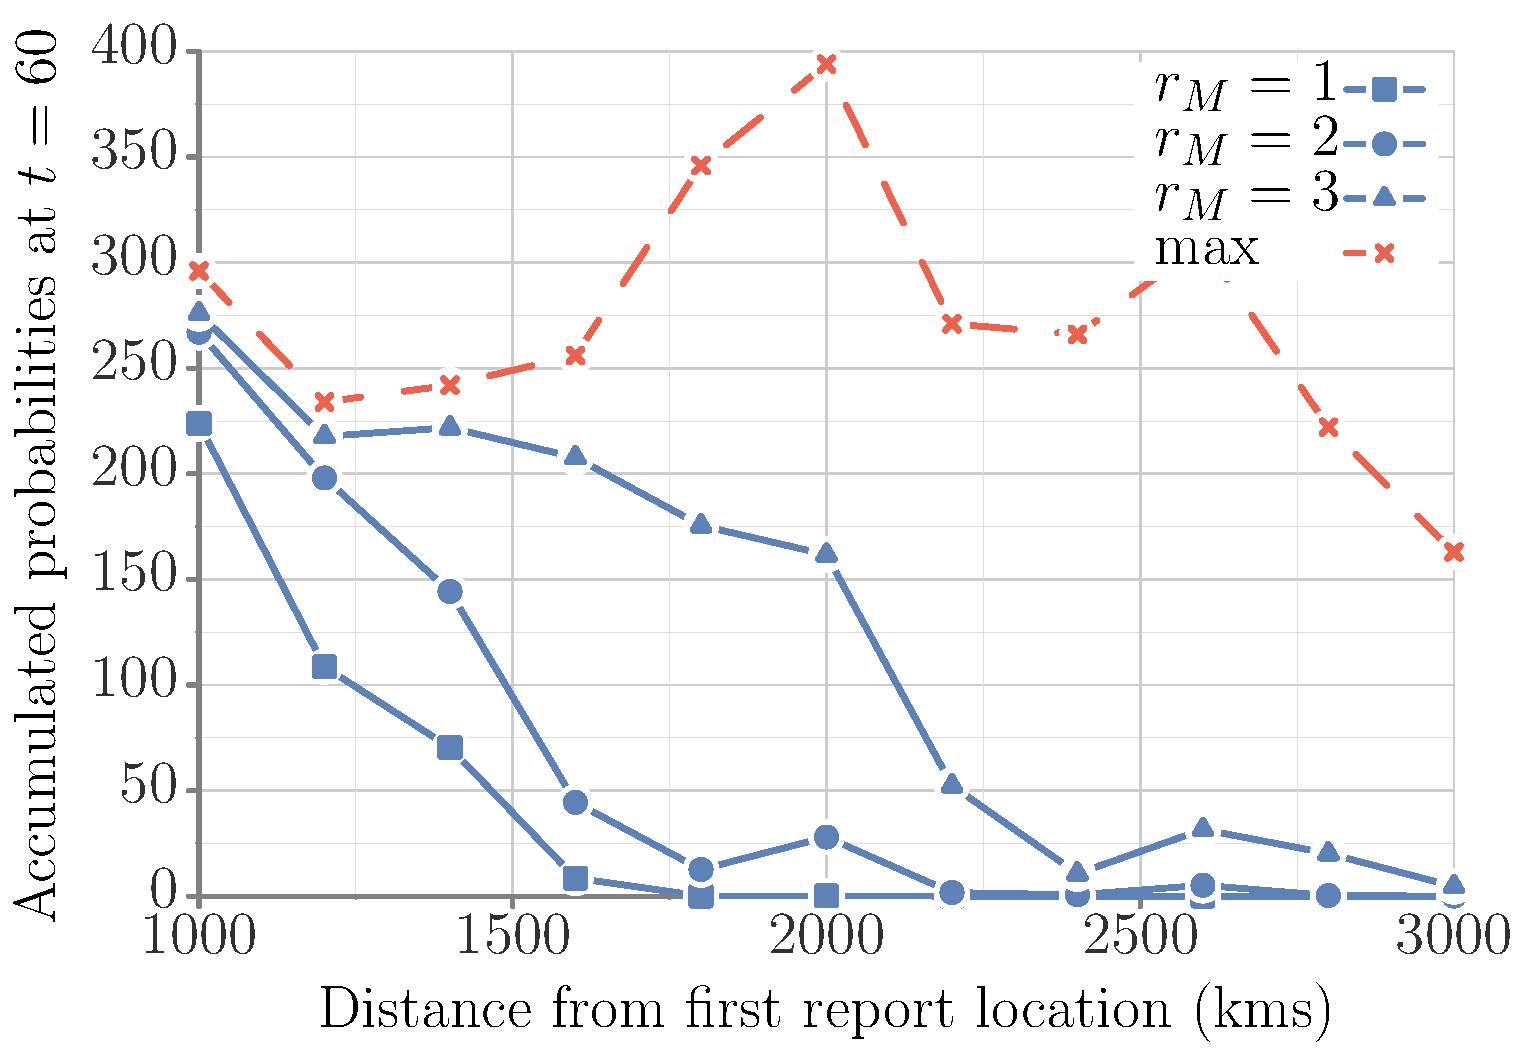
\includegraphics[width=\textwidth]{../cellular_automata/results/dist_inf_plots/dist_prob_B_moore.pdf}
%% %%     \caption{Model~A\label{fig:spreadRateMooreA}}
%% %% \end{subfigure}
%% %% %%
%% %% \begin{subfigure}[b]{.47\textwidth}
%% %%     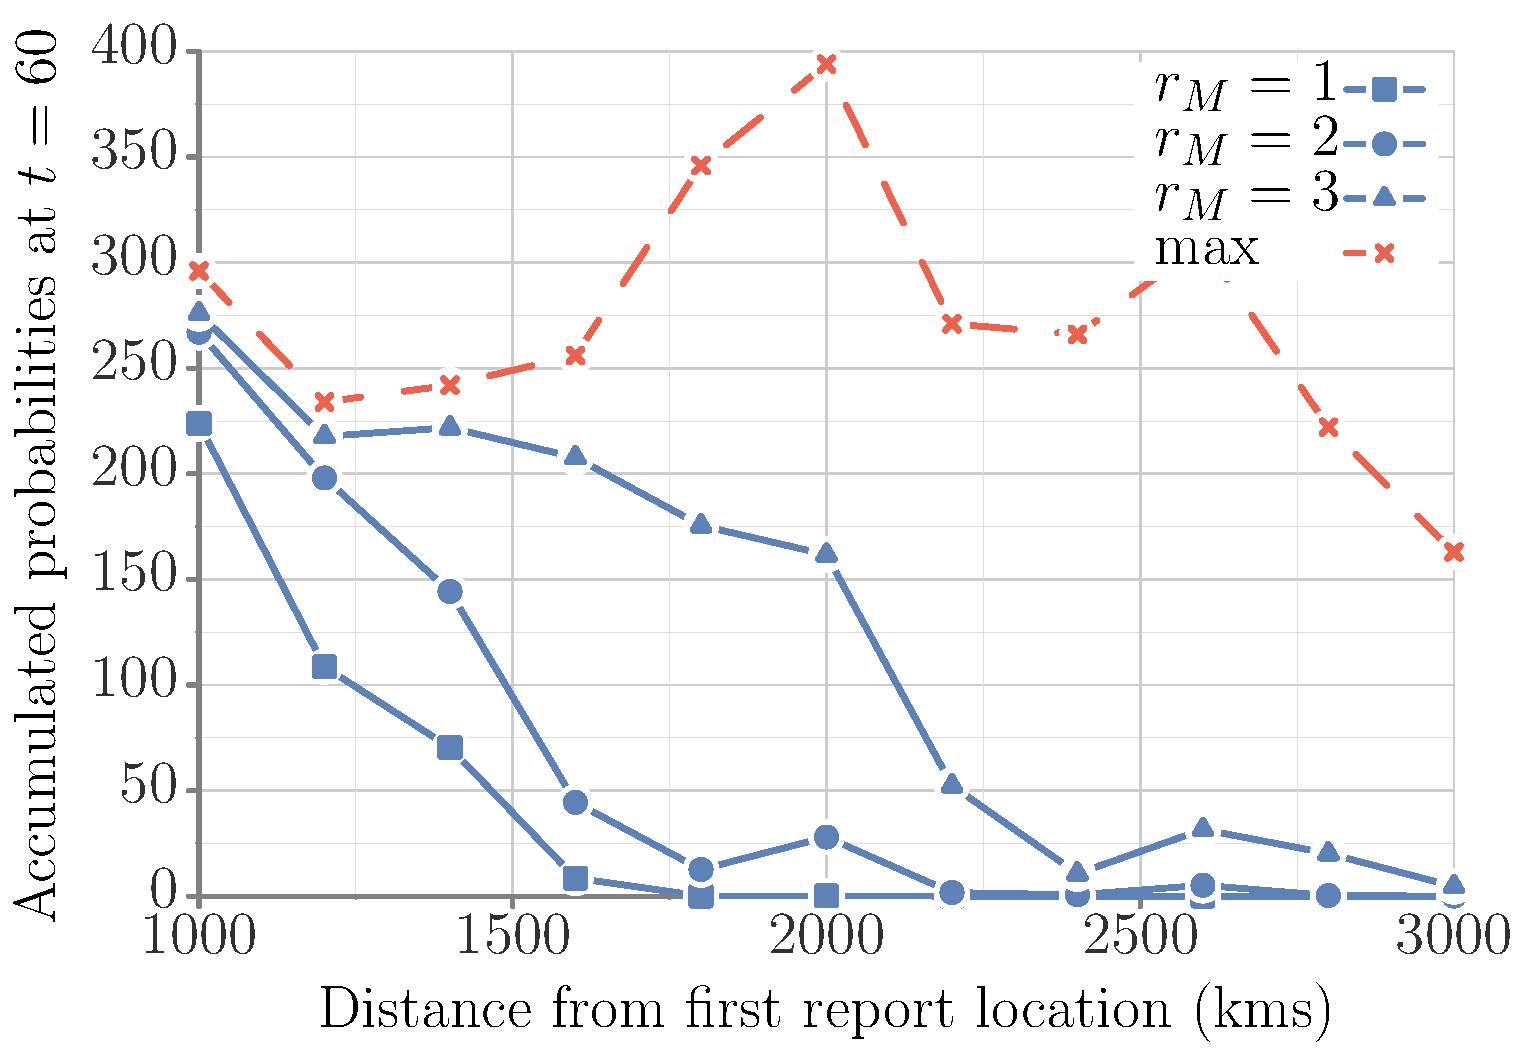
\includegraphics[width=\textwidth]{../cellular_automata/results/dist_inf_plots/dist_prob_B_moore.pdf}
%% %%     \caption{Model~B\label{fig:spreadRateMooreB}}
%% %% \end{subfigure}
%% %% %%
%% \begin{subfigure}[b]{.47\textwidth}
%%     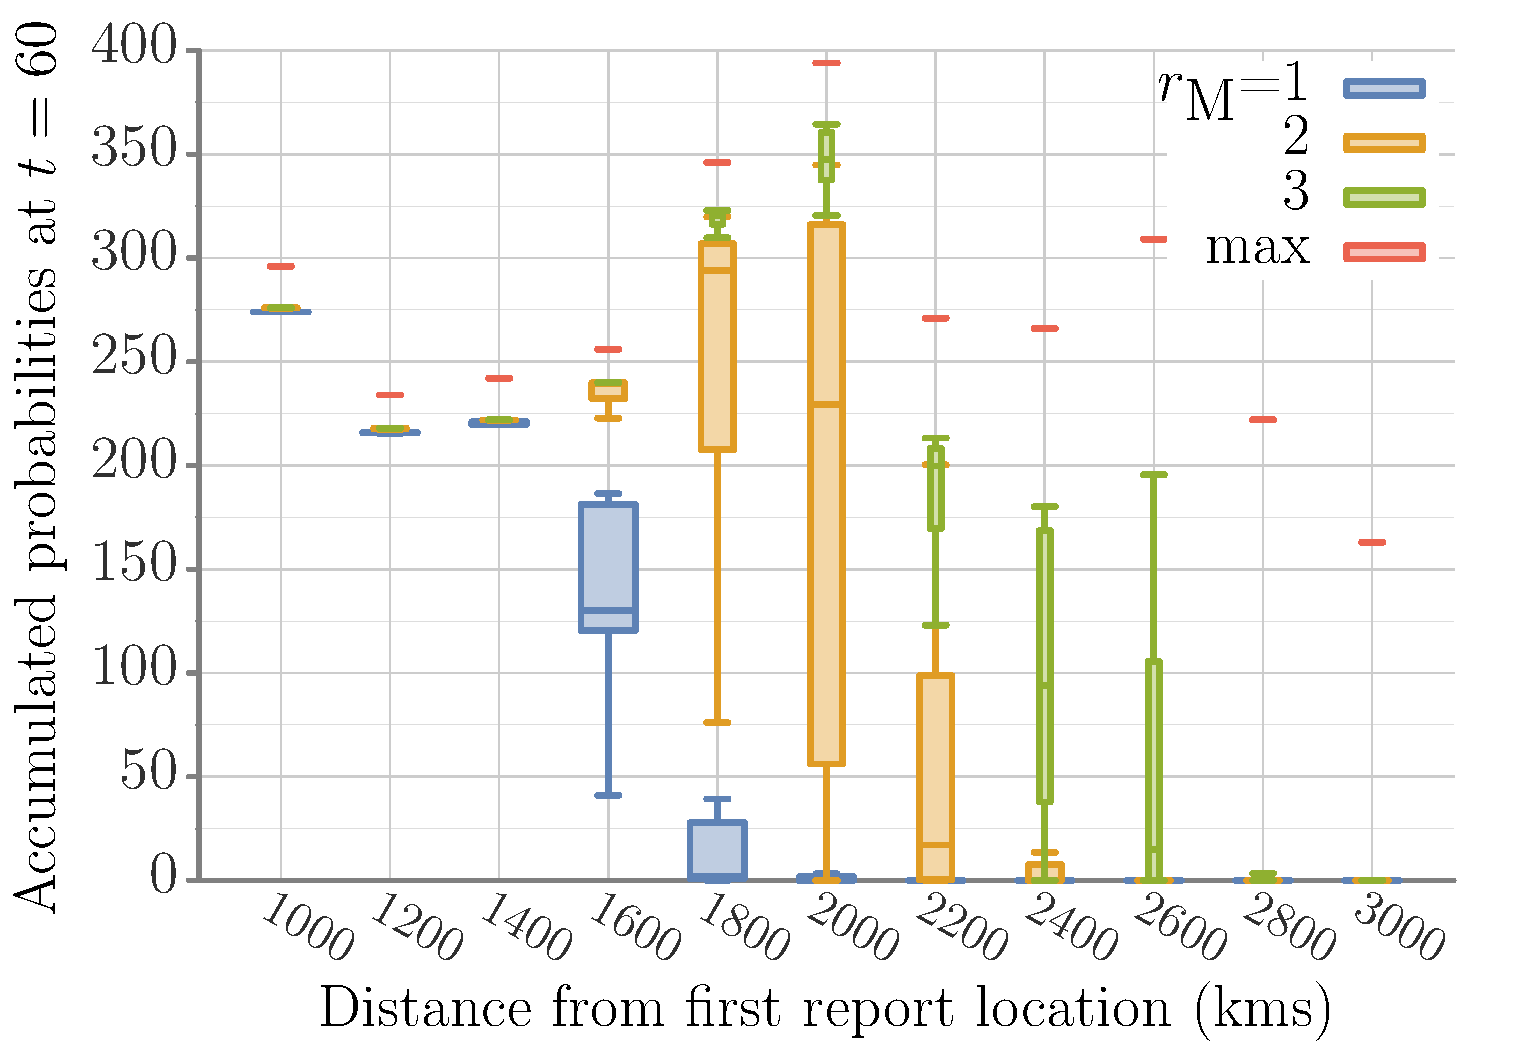
\includegraphics[width=\textwidth]{../cellular_automata/results/dist_inf_plots/dist_prob_A_box.pdf}
%%     \caption{Class~A\label{fig:spreadRateA}}
%% \end{subfigure}
%% %%
%% \begin{subfigure}[b]{.47\textwidth}
%%     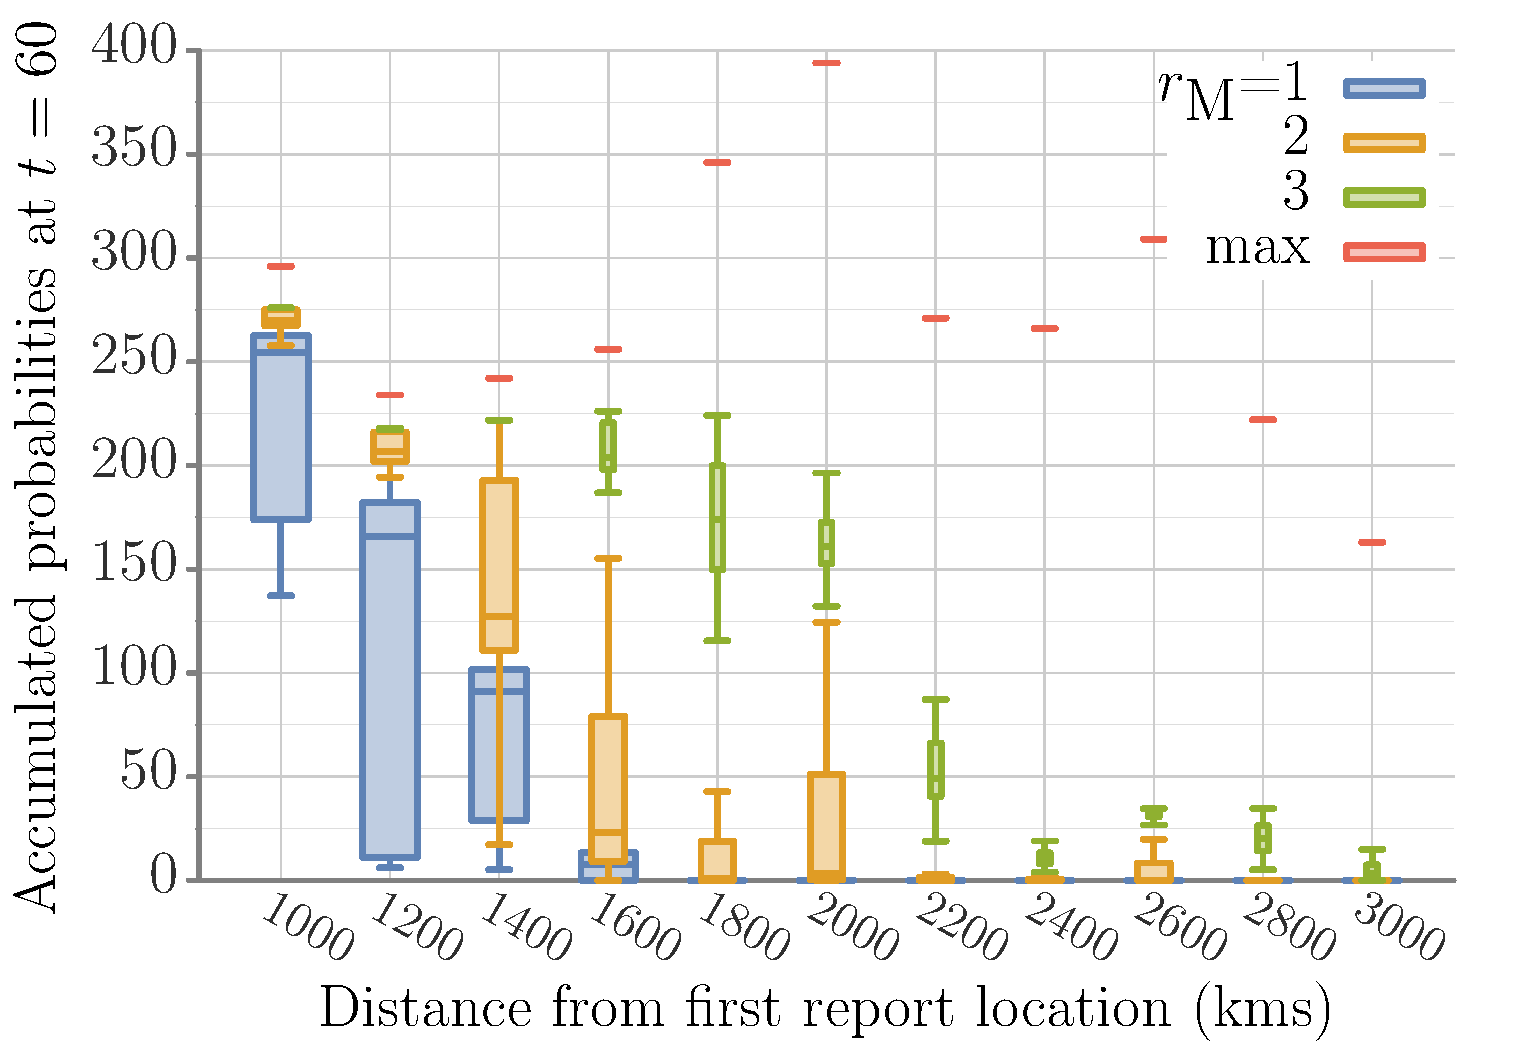
\includegraphics[width=\textwidth]{../cellular_automata/results/dist_inf_plots/dist_prob_B_box.pdf}
%%     \caption{Class~B\label{fig:spreadRateB}}
%% \end{subfigure}
%% \caption{\textbf{Spread in Mainland Southeast Asia with respect to distance
%% from origin.} The cells are binned based on their distance from the origin
%% of infection (Northern Myanmar). Given time step~$t$ (60 or five years from
%% time of start in this case), let $\Pr(v,\le t)$ be the probability that
%% cell~$v$ is in state~$I$ by time~$t$. For each parameter instance, we
%% computed the ``total infection'' for every bin at time~$t$ by
%% aggregating~$\Pr(v,\le t)$ for each~$v$ in the bin.  Parameter instances
%% were grouped by model class and Moore range ($\mooreRange$). The average
%% total infection for each group are plotted.  The red points referred to as
%% ``max'' correspond to the total number of cells in each bin, which is also
%% the maximum possible accumulated probability for that bin. We observe that
%% even though the models exhibit similar spread for Bangladesh, there is high
%% variance in spread rate in both classes for spread in in the case of he
%% spread rate when applied to the rest of the region. Also, the range of
%% expansion is influenced by Moore range~$\mooreRange$.
%% \label{fig:spreadRate}
%% }
%% \end{figure}
%%

%% To account for possible increase in production and trade, we boosted the
%% pathway parameters by (i)~25\% and (ii)~50\%. The results in
%% Figure~\ref{fig:spreadRate} show the increase in intensity of infection,
%% but not an appreciable increase in range.

%%
\paragraph{Alternate scenarios of invasion.}
From the analysis of the international trade network
(Figure~\ref{fig:tomnet}), we observe that Malaysia and Singapore are
important hubs with tomato imports from \tuta{} infested regions. There is
a possibility that \tuta{} is directly introduced to these regions. However,
as mentioned earlier, the import volume is very low. Also, the introduction
risk depends on the preventive measure taken by the exporting countries.
Nevertheless, we considered the scenario in which \tuta{} establishes in the region
between Kuala Lumpur and Singapore. The simulations suggest that the pest
will spread to most localities in Malaysia and Sumatra, Indonesia within an
year.

The second scenario we considered is the introduction of \tuta{} to
Philippines. Since Philippines does not share its borders with any country in the region
and there is no evidence of tomato trade with rest of the countries, there
is a low chance that the pest will be introduced through natural spread or
trade.  However, human mobility is a possible pathway. The Middle East is
the top destination for Filipino workers~\cite{rodriguez2011philippine}.
Therefore, there is a possibility of introduction through travel. We
considered two hypothetical scenarios: (i)~\tuta{} is introduced to the Palawan region
from Malaysian Borneo and (ii)~it is introduced to the high production area
of Northern Mindanao. While in the first case we did not observe spread
beyond the Palawan region, in the second case, within two years, almost all
localities were invaded. The latter case is shown in
Figure~\ref{fig:phlBContour}.
%%
\paragraph{Interventions at the trade level.}
Given that monitoring and quarantining are both resource intensive and
potentially disruptive, developing strategies that involve few locations,
yet provide near-optimal control is a goal for modelers. 
Market-level phytosanitary measures in terms of import restrictions have
been undertaken by countries~\cite{USDA2012}. Here, we evaluated a simple
strategy of containing the spread through the trade pathway. Localities
associated with high annual outflows were identified. As discussed earlier,
pest establishment in these areas can potentially lead to rapid range
expansion. The outflow from the targeted localities was cut off to mimic
control at the trade/market level. Note that cutting off outflow does not
necessary imply restricting trade of host crops. It is possible that
phytosanitary measures greatly reduce the chance of spread through trade.
Firstly, we identified localities with high outflows (at most four in each
country).  Figure~\ref{fig:spread} shows results for two countries. More
results are present in Figure~\ref{S:fig:intervene} in the supplement.
Consistently, across countries, we observed a significant reduction in
range expansion as well as intensity of spread.  Besides, as seen in
Figure~\ref{fig:thlBContourInt}, stifling these flows leads to a local and
more importantly, predictable spread pattern that resembles those of
Class~A models, but with much less intensity. 
%%
%% Given the importance of the long-distance human-mediated pathway, we
%% studied the effect of controlling this pathway in mitigating the spread.
%% Monitoring localities by setting up pheromone traps in production areas and
%% markets, and quarantining affected areas is one way to accomplish this.
%%
\begin{figure}[ht]
\begin{subfigure}[b]{.28\textwidth}
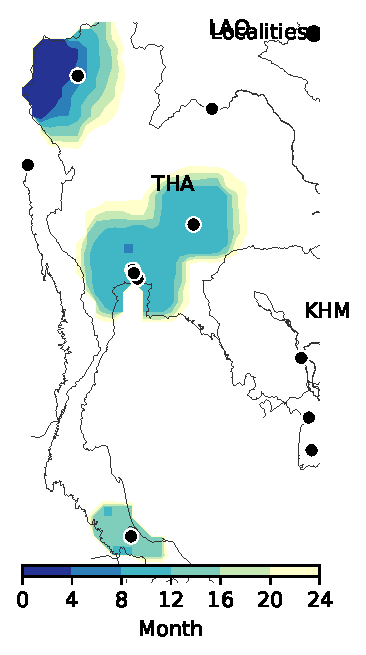
\includegraphics[width=\textwidth]{../cellular_automata/results/contour/TH_model-B_precip1_m1_l3.pdf}
\caption{Thailand without intervention\label{fig:thlBContour}}
\end{subfigure}
\begin{subfigure}[b]{.28\textwidth}
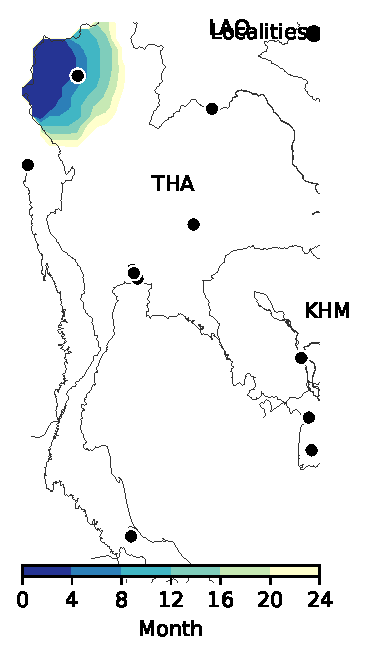
\includegraphics[width=\textwidth]{../cellular_automata/results/contour/TH_model-B_precip1-out-100_m1_l3.pdf}
\caption{Thailand with intervention\label{fig:thlBContourInt}}
\end{subfigure}
\begin{subfigure}[b]{.43\textwidth}
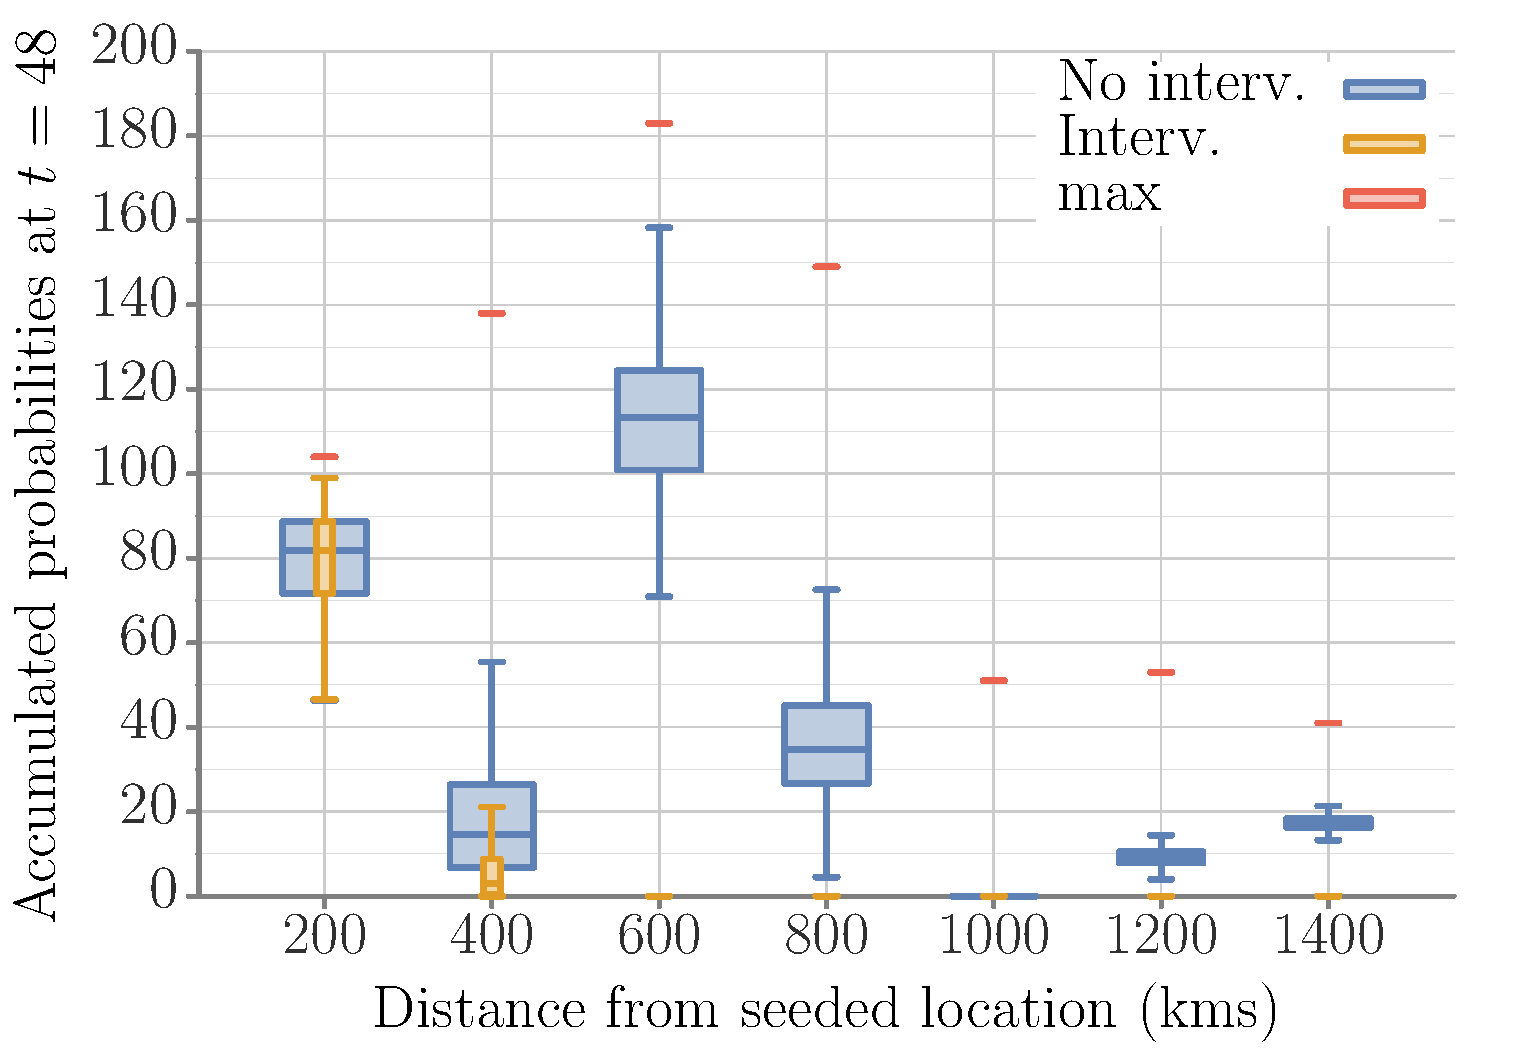
\includegraphics[width=\textwidth]{../cellular_automata/results/dist_inf_plots/TH_dist_prob_B_box.pdf}
\caption{Thailand: range of expansion (all Class B models)\label{fig:thlBContourBox}}
\end{subfigure}
\begin{subfigure}[b]{.28\textwidth}
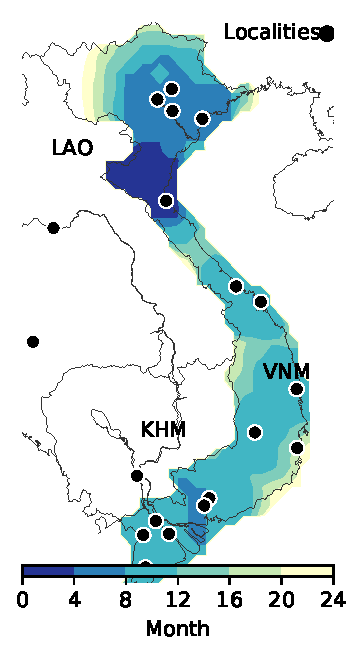
\includegraphics[width=\textwidth]{../cellular_automata/results/contour/VN_model-B_precip1_m1_l3.pdf}
\caption{Vietnam without intervention\label{fig:vnmBContour}}
\end{subfigure}
\begin{subfigure}[b]{.28\textwidth}
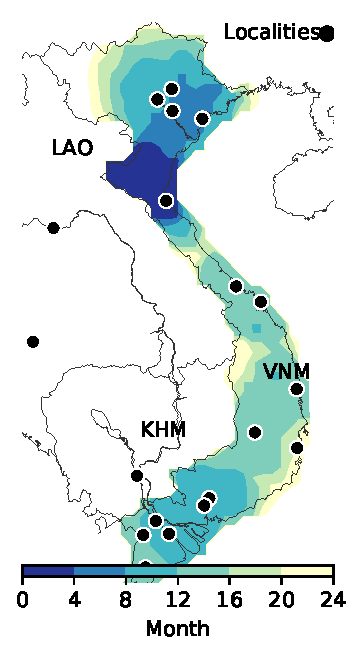
\includegraphics[width=\textwidth]{../cellular_automata/results/contour/VN_model-B_precip1-out-100_m1_l3.pdf}
\caption{Vietnam with intervention\label{fig:vnmBContourInt}}
\end{subfigure}
\begin{subfigure}[b]{.43\textwidth}
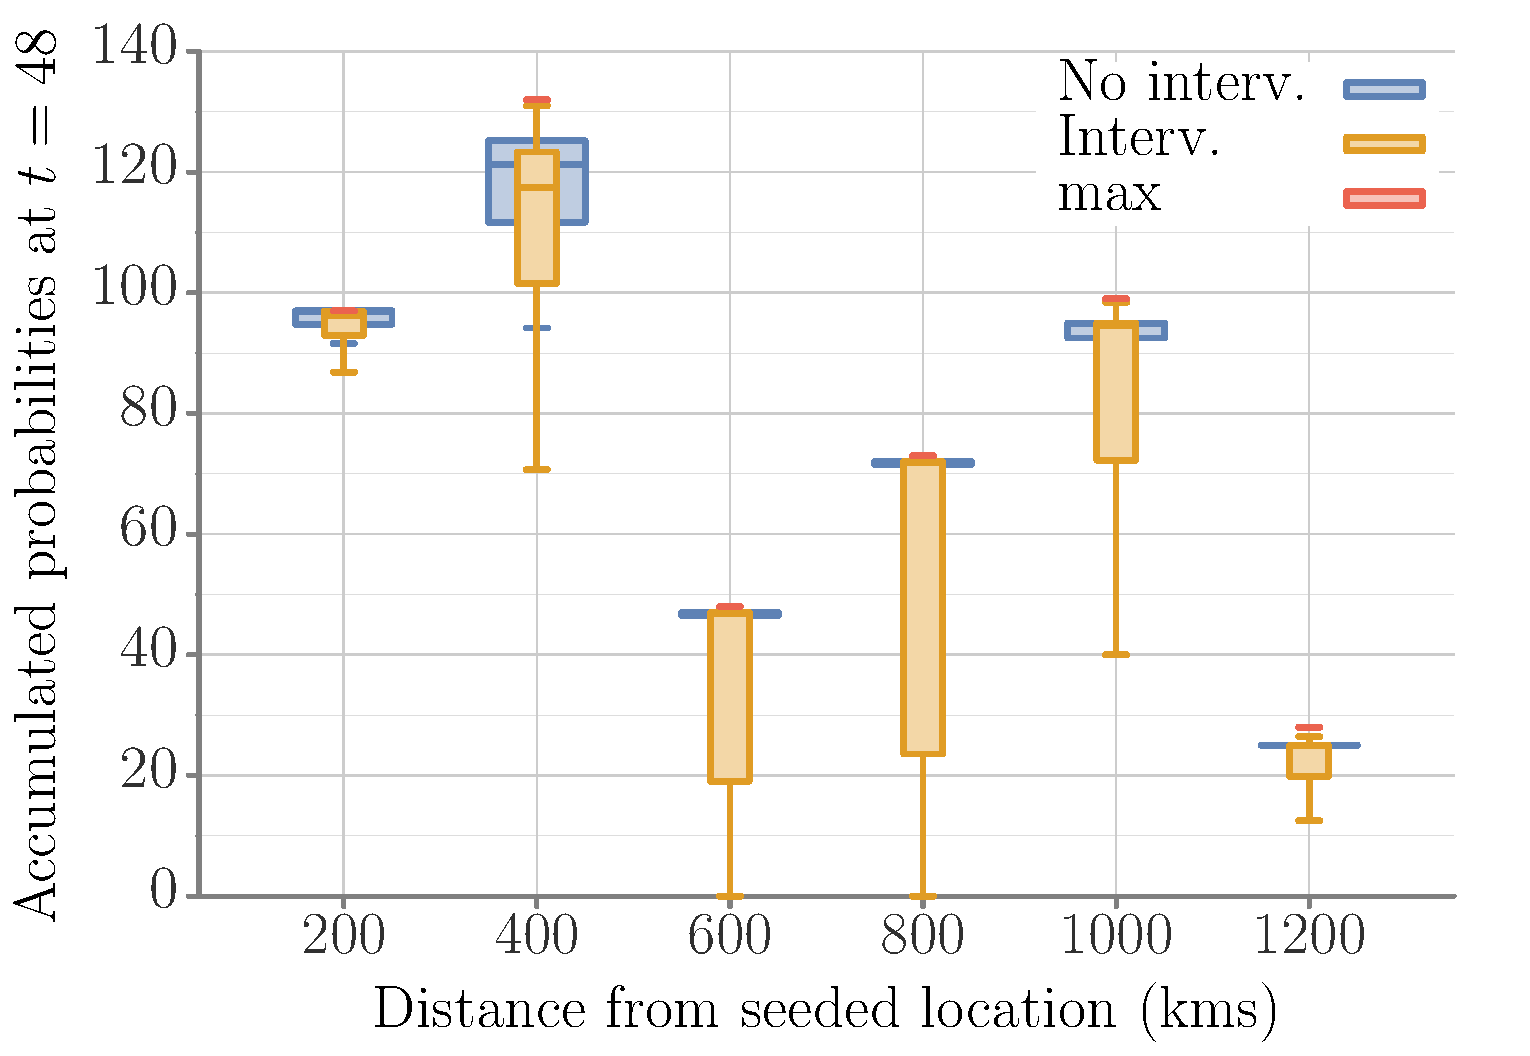
\includegraphics[width=\textwidth]{../cellular_automata/results/dist_inf_plots/VN_dist_prob_B_box.pdf}
\caption{Vietnam range of expansion (all Class B models)\label{fig:vnmBContourBox}}
\end{subfigure}
\caption{\textbf{Rate and pattern of spread with and without intervention.}
Representative spread dynamics of Class~B models ($\mooreRange=1, \ell=3$)
for two countries. More plots are in Figure~\ref{S:fig:intervene}. In each
case, a cell close to a high production region was seeded. The first column
corresponds to spread for 48 months after introduction. The colors indicate
the time interval at which there is at least a 50\% chance that a location
will be infected.The second column corresponds to spread after cutting off
flows from chosen localities. The third column shows average spread with
respect to origin of infection for all Class~B models.
\label{fig:spread}}
\end{figure}
%%     \textbf{Interventions.} The effect of
%% reducing outflows from major production regions is shown for Class~B
%% models. These are representative results for Philippines. Plots for other
%% countries are in Figure~\ref{S:fig:intervene}. In the simulations, a high
%% production region (Northern Mindanao) was seeded. (a)~\textbf{Without
%% intervention.} Simulations indicate that for the given initial conditions,
%% there is a high chance that all major production areas of Philippines will
%% be affected within 24 months.  The colors indicate the time interval at
%% which there is at least a 50\% chance that a location will be infected.
%% (b)~\textbf{With market level intervention.} The spread without the
%% influence of long-distance flows from localities corresponding to high
%% production areas (Northern Mindanao and Central Luzon). We observe a delay
%% of more than two years in the introduction to the northern part due to this
%% intervention.  (c)~\textbf{Spread with respect to origin of infection.}
%% We compare the effect of reducing the long-distance flow the
%% above-mentioned regions by 50\% and 100\%. The results shown correspond to
%% all Class~B instances with Moore range~$\mooreRange=1$. \label{fig:intervene}}
%% Under the assumption that appropriate control
%% measures are taken, we reduce the incoming and outgoing edge weights
%% by~$50\%$ of their original value. The resulting model was compared with
%% the case where no action is taken (Section~\ref{sec:predict}).
%% 
%% Farm-level \aacomment{not sure about this}
%% \begin{itemize}
%%     \item suitability threshold is varied
%%     \item Scenario 1 where for all cells it is done
%%     \item Scenario 2 where for it is done in key tomato growing areas
%%     \item Scenario 3 where it is done only near localities
%% \end{itemize}
%% 
%% Market-level
%% \begin{itemize}
%%     \item Scenario 1: we identify localities which are hubs (lots of
%%     outflow) and reduce their flow.
%% \end{itemize}
%% %%
%% \begin{figure}[ht]
%%     \centering
%%     \begin{subfigure}[b]{.47\textwidth}
%%         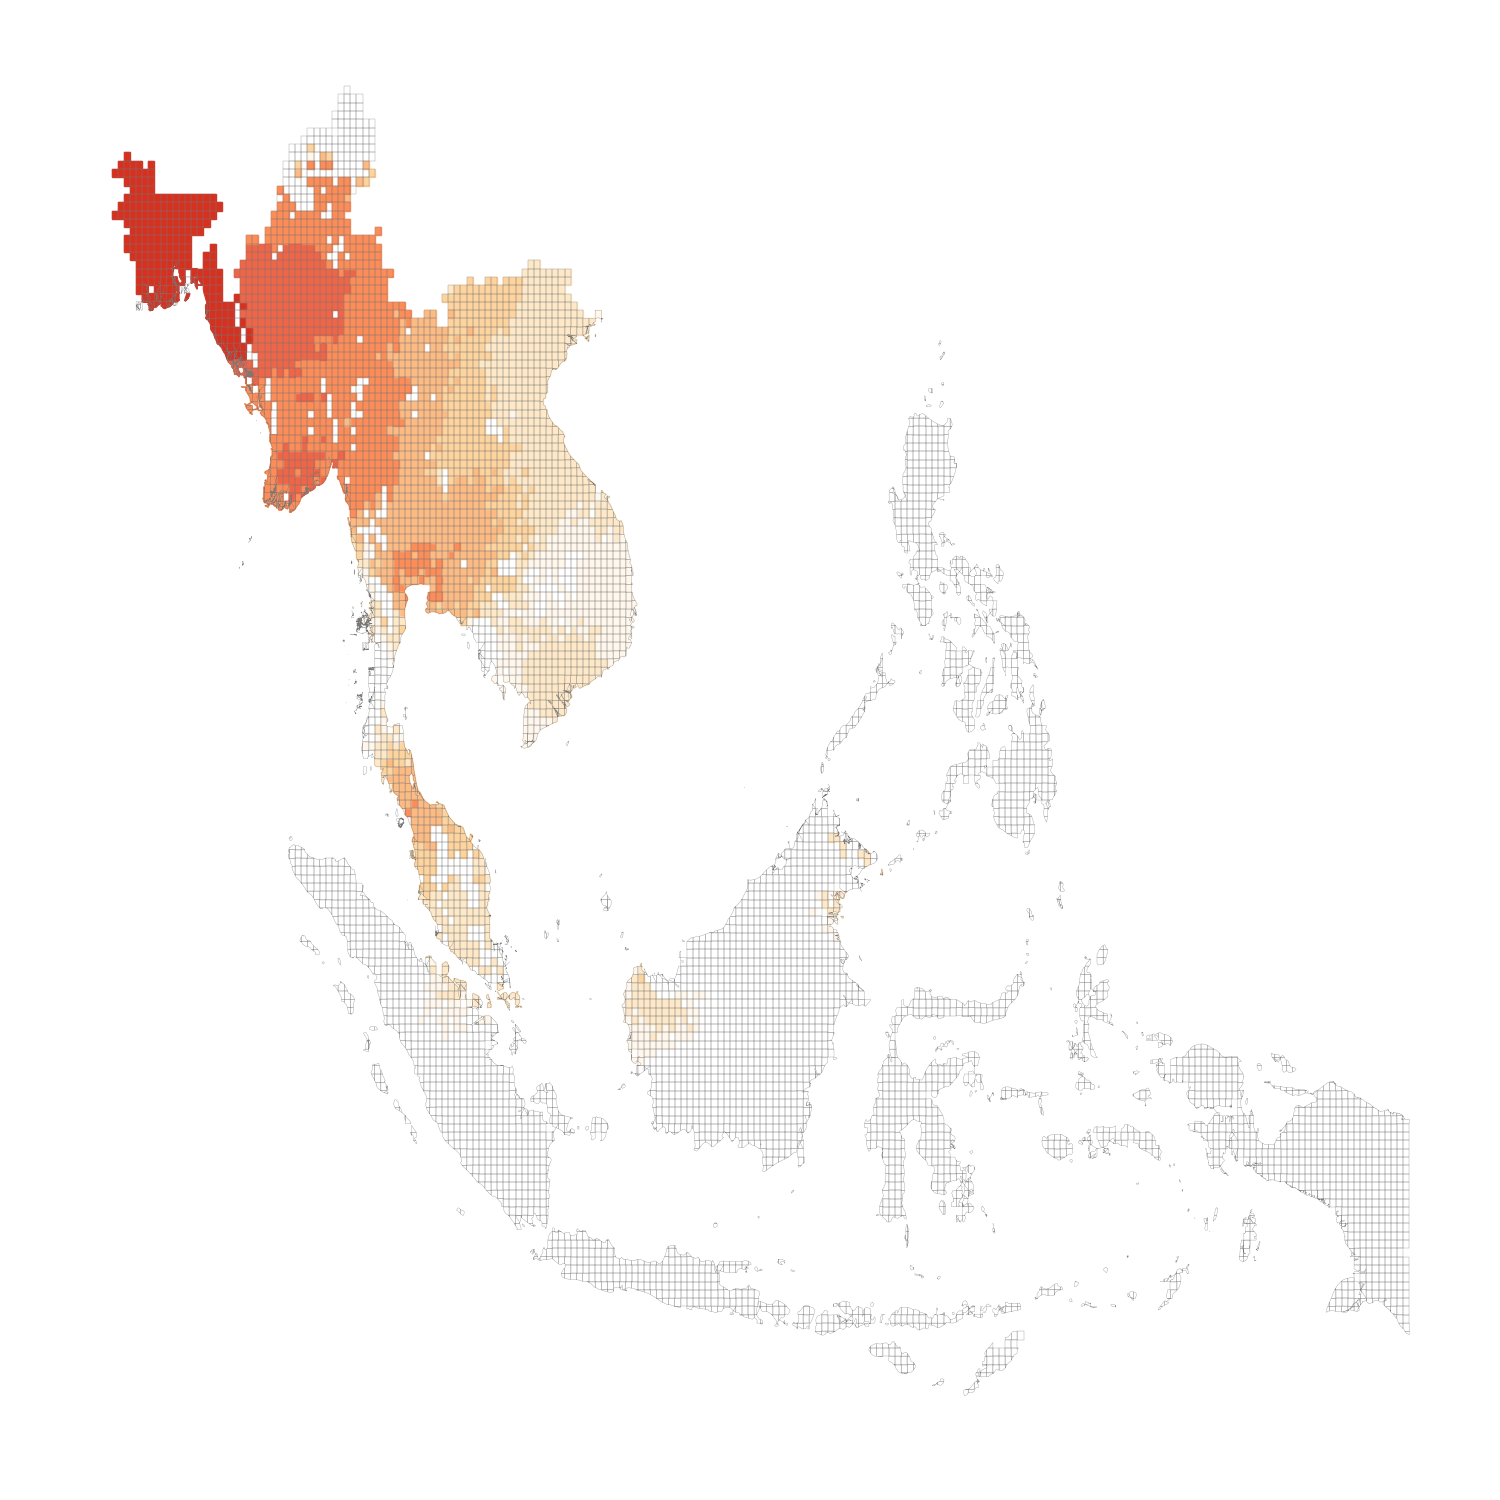
\includegraphics[width=\textwidth]{figs/spread_farm_level_interventions.png}
%%     \caption{\label{fig:spreadFarmLevel}}
%%     \end{subfigure}
%%     \begin{subfigure}[b]{.47\textwidth}
%%     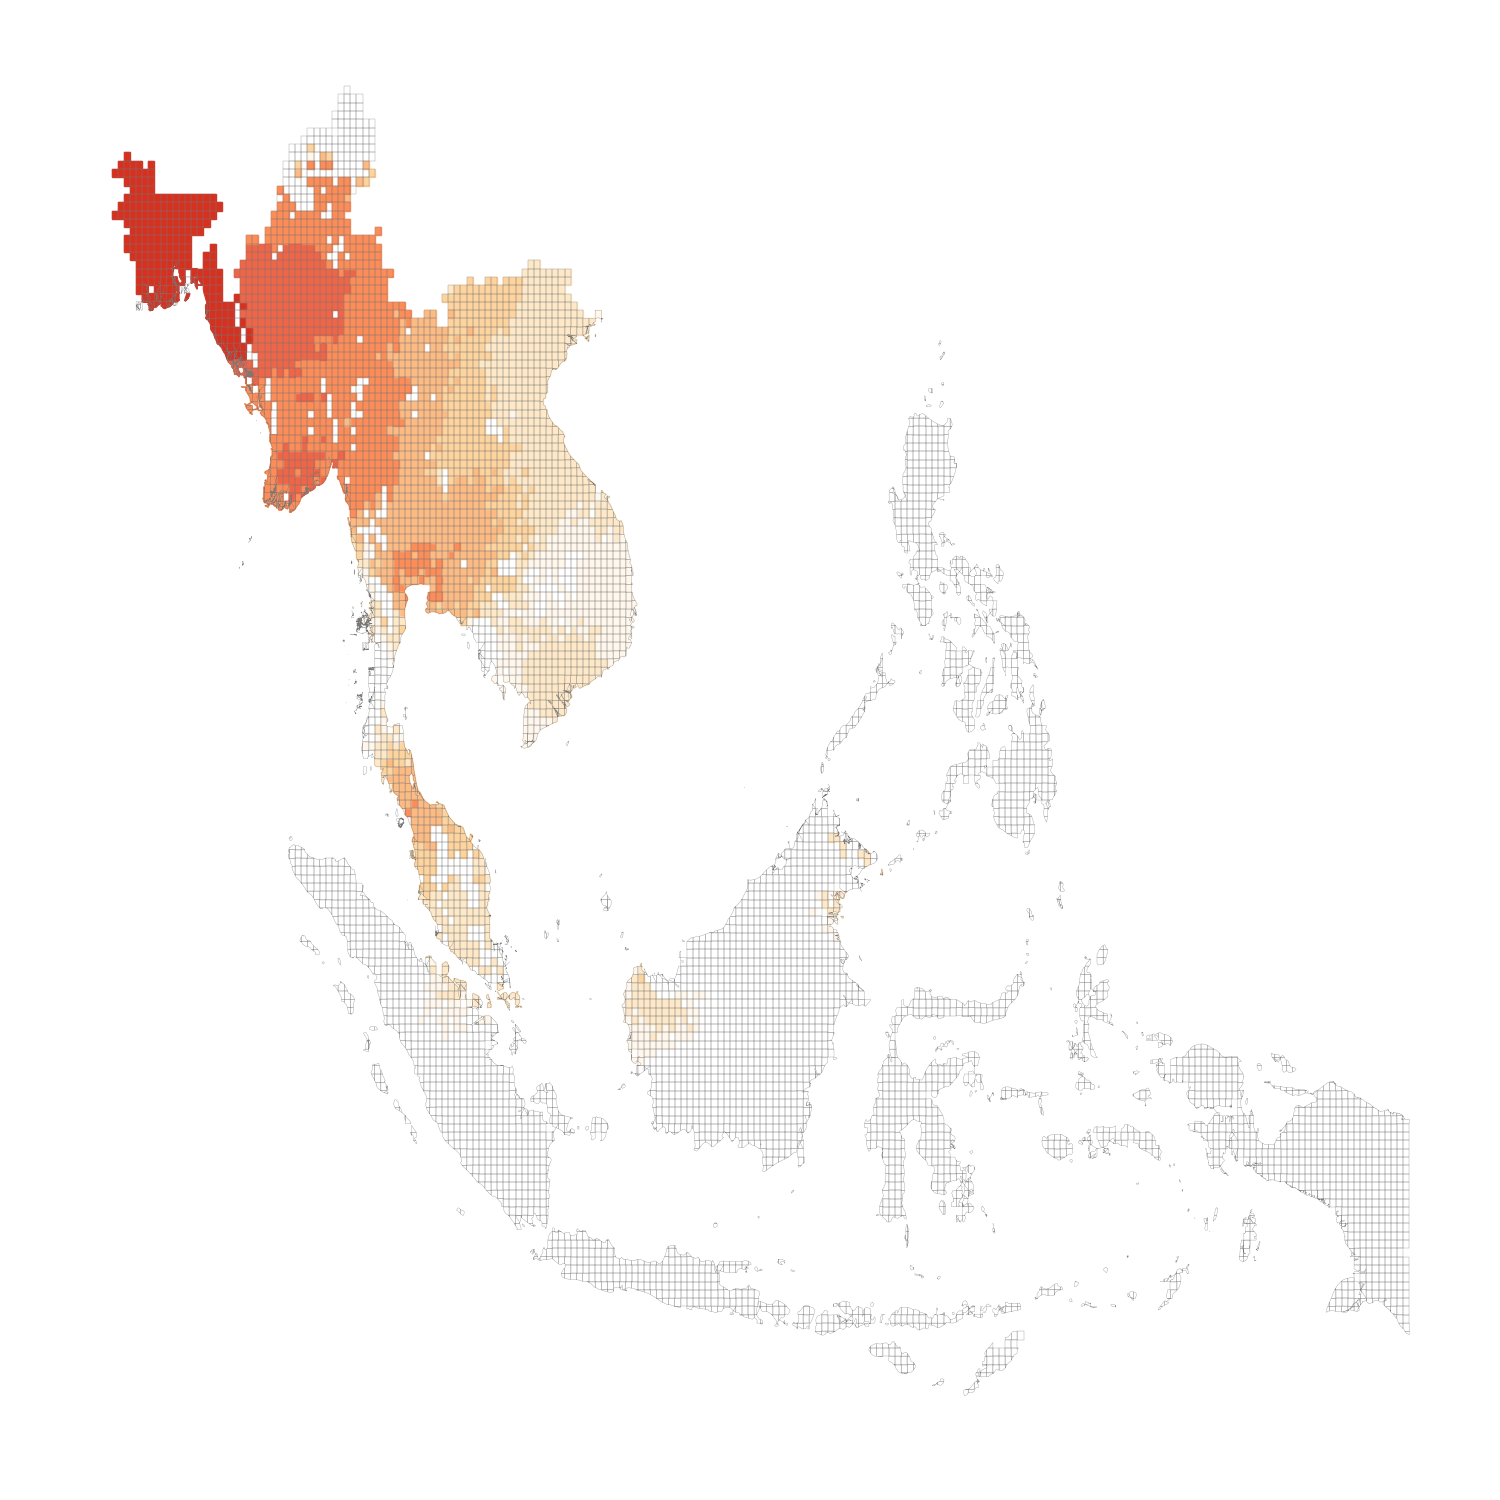
\includegraphics[width=\textwidth]{figs/spread_market_level_interventions.png}
%%     \caption{\label{fig:spreadMarketLevel}}
%%     \end{subfigure}
%%     \caption{Effect of interventions}
%% \end{figure}

%%
\section{Discussion}


need to say take away points
\begin{enumerate}
    \item need sample flows for calibration. need to study heterogeneity
    \item need function for relation between flow and pest spread
    \item what is enough for modeling trade? at minimum what is
    required?
    \item SIS Epidemics in Multilayer-based Temporal Networks
\end{enumerate}
other stuff
\begin{enumerate}
    \item bias in sampling
    \item feedback not accounted for
    \item others have only considered smaller area
\end{enumerate}

The multiple expl 

    flying capability is important to consider given class A and
    class B models

    model uncertainty
It is possible that we have not accounted for
long-distance flows that might explain this spread. A more plausible
explanation is that a second invasion happened from India. In January 2017,
\tuta{} was reported from Umiam~\cite{sankarganesh2017}, Meghalaya about
100kms from Jaintiapur.  It also happens to be near an important trade
route from India to Northeastern Bangladesh.

\paragraph{Impact.} Traditionally, crops such as tomato have been grown in
the dry season, which is usually during winter in most parts of Southeast
Asia. However, over the past decade, due to rising demand and opportunities
to export, there has been a thrust towards year-round production using
protected cultivation methods and resilient varieties~\cite{ali2001}.
Tomato production and internal trade has steadily increased in this region
(See Figure~\ref{S:fig:trends} in supplement). In comparison, the export of
tomato to outside of the focus region has risen steeply in the recent years
(after 2011), while the imports generally indicate a downward trend.
Therefore, invasions from pests such as \tuta{} can have a huge negative
impact on the socioeconomic fabric of this region.  Although there is a
general consensus that vegetable and seedling trade is a primary driver of
\tuta{} spread, previous modeling efforts have exclusively focused on
ecological aspects. Several
studies~\cite{desneux2010biological,tonnang2015identification} provide risk
maps using CLIMEX and take additional factors into account.
Guimapi~et~al.~\cite{guimapi2016modeling} used a cellular automata approach
to capture the global spread of the pest by factoring in temporal
variations and spatial distribution of vegetation, temperature, and tomato
production. A precursor to this work~\cite{venkatramanan2017towards}
modeled the seasonal production and trade of tomato in Nepal to study the
role of trade in the spread of \tuta{} in Nepal using gravity model and
network dynamics.
%% A novel ranking-based
%% inference was used to establish that trade was indeed a driving factor in the
%% rapid spread of the pest in this region.
%% In general, modeling the multi-pathway dispersal of pests such as \tuta{}
%% is a challenging task due to inadequate understanding of the complex
%% interconnected food system. To add to the
%% problem, most countries ended up not being prepared for the infestation,
%% either due to lack of awareness of the pest or the sheer speed of invasion.
%% Absence of quality incidence records makes callibration and validation
%% hard. Some of these problems were highlighted in the modeling
%% effort by 

%% In recent years, there has been a thrust towards integrated modeling
%% approaches to understand invasive species dynamics. 
%%
\paragraph{Literature survey.} Multi-pathway models are being increasingly
used to study the role of invasive species dispersal.
Douma~et~al.~\cite{douma2016pathway} survey the literature categorizing
various efforts into flow-based pathway models and agent-based models.
Robinet~et~al.~\cite{robinet2009role} show that the distribution and spread
pattern of the pinewood nematode in China is strongly correlated with
density of human population and infrastructure such as railways and river
ports.  Carrasco~et~al.~\cite{carrasco2010unveiling} combine spatially
explicit models with a phenology model to incorporate population dynamics
of the pest (western corn rootworm). Two types of long-distance dispersals
are considered -- domestic and international. The domestic mode is modeled
as a flow network between cities using a gravity model approach.
Nopsa~et~al.~\cite{nopsa2015ecological} use a network science approach to
studying the role of transport and storage infrastructure in the spread of
pests and pathogens of wheat. Sutrave~et~al.~\cite{sutrave2012identifying}
use a time-varying network model to study the spread of Soybean rust.  Our
model is in part motivated by the hybrid approaches used in the study of
infectious diseases of humans and livestock.
Bradhurst~et~al.~\cite{bradhurst2015hybrid} study the spread of foot and
mouth disease in livestock by using an aggregate population-level model to
capture within-herd spread and an individual-based model for between herd
spread. A similar approach is used by Yang~et~al.~\cite{yang2016} to
forecast influenza outbreaks. They use a patch network model where a
compartmental model is used to simulate intra-locale spread and a gravity
model based approach is used for inter-locale spread of flu in the
neighborhoods of New~York.

%% The modeling framework developed in this paper can
%% be used to study the spread of \tuta{} in other regions. However, it is
%% possible that additional factors need to be accounted for. 
%% It can also be applied to other pests. However, this would require first
%% assessing the importance of each pathway based on evidence: diapause and flying
%% capacity, spread by human mobility or trade, etc.  

Our results suggest that intervening at the trade level is very effective
in stiffling the spread. While, several IPM strategies have been suggested
for managing \tuta{}, hardly any work has been done in designing effective
interventions at the trade level. Designing phytosanitary measures
targetted towards market and vehicles of transportation for preventing
introductions (or reintroductions) is therefore a promising research
direction. Some countries have already taken measures in this regard. The
Animal and Plant Health Inspection Service of the United States Department
of Agriculture (USDA-APHIS) has instituted quarantine regulations for
imports from regions where the pest is present~\cite{USDA2012}. Identifying
the optimal set of nodes in a network to reduce infectious disease spread
is a widely studied topic~\cite{madar2004immunization}. There are very few
works that apply such techniques to invasive species spread.
Nopsa~et~al.~\cite{nopsa2015ecological} considered this problem in the
context of soybean rust in the US, modeling the spread as a propagation
process over a network of counties. They developed efficient strategies to
reduce the spread by identifying and monitoring only a subset of locations
which are critical for the spread.


\paragraph{Challenges and limitations.}
Modeling emerging invasions is particularly challenging. Accounting for
multiple pathways of spread inevitably increases model complexity. On the
other hand, limited data on incidence and understanding of the underlying
dynamics makes it nearly impossible to calibrate and validate the models.
Besides, since our focus region spans multiple countries, identifying and
collecting data for each country was a tedious process. For many countries,
data had to be collected (or even inferred) from several publications and
reports (Table~\ref{S:tab:countryData}). Further, these datasets were
misaligned in time and spatial resolution. We have had to simplify or
ignore some of the processes that might significantly influence the spread.
For example, our model uses monthly production as a surrogate for
infectiousness of a cell. Complex phenology models can be used instead (as
in Carrasco~et~al.~\cite{carrasco2010unveiling}). While such a model for
\tuta{} would be useful, this would add to the complexity of
the model~\cite{robinet2012suite}.
%%
%% multi-pathway model incorporated a multitude of
%% datasets-- production, consumption, trade dynamics, climate, biology, etc.
%% On the other hand, 
%% To capture the
%% multi-pathway dynamics complexity of
%% invasion dynamics demands the use of several datasets spanning mulitple
%% domains.
%% Hence, we have had to simplify or ignore some of
%% the processes that might significantly influence the spread.
%% amid data scarcity and
%% heterogeneity. makes modeling has forced
%% us to simplify or ignore some of the processes that might
%% significantly influence the spread. 
%%

In particular, it is hard to model human assisted spread owing to lack of
seasonal trade data. Production is dependent not only on the host, climate,
and geography, but also on people's preferences and market demand. To
determine outflows and inflows for each locality, we had to identify major
ports for imports and exports as well as estimate fraction of production
which was used for processing. This data was available only for a few
countries.  The farm--market-consumer interactions (local human-mediated
spread) involves various actors such as farmers, wholesalers, retailers,
wet markets, supermarkets, etc. Modeling this is a challenge in itself. If
data on actual flow of vegetables is provided, the gravity model can be
improved or replaced by more sophisticated approaches. Also, the
relationship between long-distance invasion risk and trade volume is hard
to determine. While a direct relationship between volume and risk is
plausible, whether the relation is linear (as assumed by our model) is not
clear.

%% Therefore, data came from disparate sources, and were misaligned in time
%% and spatial resolution. Production and trade data from FAOSTAT also had
%% gaps in them.  
%% The fidelity of models such as the one presented here crucially depends on
%% the availability of quality data as well as a good understanding of the
%% processes involved. 
%% Another example is the modeling of consumption.
%% It is possible that there is lot of variation in consumption within a
%% country~\cite{wijk2007} as well as across seasons. Even at the country
%% level, data is available for only half of the countries. Also, we did not
%% find any correlation between consumption and GDP or tomato production
%% (correlation $< 0.01$).  to model accurately the growth
%% of the pest under specific conditions including the tritrophic interactions
%% concerning the pest, host, and its indigenous predators
%% Rebaudo~et~al.~\cite{rebaudo2011}, for example, use a complex
%% agent-based model to study just the interaction between farmers of two
%% villages in the context of the potato moth in Ecuador. 

It is important to account for heterogeneity in production, consumption,
awareness, cultural factors, etc. both within and between countries. Some
countries are technologically more advanced than others, which manifests as
differences in yield, crop loss, trade infrastructure, pest awareness and
preparation for invasion~\cite{early2016global}. It is possible that there
is lot of variation in consumption within a country as well as across
seasons. The relationship between trade volume and distance between
localities could vary from one region to another. Extending to other
regions such as North America, China or Australia, might require accounting
for seedling trade and greenhouse production.
%% Even at the country level, data is available for only half of the
%% countries. Also, we did not find any correlation between consumption and
%% GDP or tomato production ($p< 0.01$).  Without adequate data, it is
%% difficult to account for such heterogeneity.

\paragraph{Conclusion.} We developed a generic networked modeling framework
to understand invasive species spread accounting for self- and
human-mediated pathways. Machine learning techniques were used to address
data sparsity and model uncertainties. The model was applied to study the
spread of \tuta{} in the region of Southeast Asia. Our results suggest that
trade of host plants plays an important role in the spread of the pest.
Monitoring and control of this pathway can significantly mitigate the
spread. The methodology uses open-source datasets and can be applied to
other invasive species and host crops. Besides invasive species spread,
other potential applications for this work include studies of natural or
human-initiated disasters, climate change and optimization of food flows.

%% applying this generic modeling approach to other study regions such as
%% North America or Australia would require taking additional
%% factors into account. For example, seedling trade could be an important pathway. From a
%% production perspective, it is becoming important to factor in protected
%% cultivation methods, which have enabled farmers to extend the growing
%% season.
%% However, the developed framework is modular and extensible. Given
%% high-resolution accurate datasets and a better knowledge of the processes,
%% individual modules can be replaced with more sophisticated modeling
%% approaches.  
\paragraph{Data availability.} The authors declare that the data supporting the
findings of this study are available within the paper and its Supplementary
Information file, or from the authors upon reasonable request.

\paragraph{Acknowledgments}
This work was supported in part by the United States Agency for
International Development under the Cooperative Agreement NO.
AID-OAA-L-15-00001 Feed the Future Innovation Lab for Integrated Pest
Management, DTRA CNIMS Contract HDTRA1-11-D-0016-0001, NSF BIG DATA Grant
IIS-1633028, NSF DIBBS Grant ACI-1443054, NIH Grant 1R01GM109718 and NSF
NRT-DESE Grant DGE-154362.  We are grateful to Yousuf Mian, Nguyen Van Hoa,
and Kimhian Seng for their help with obtaining country-specific information
on production, trade, and pest incidence. We thank Richard Beckman and
Irene Eckstrand for useful discussions on model design and paper
organization.

\paragraph{Author contributions.}
AA defined the scope of the
research. AA, JM, TB, MRC collected and interpreted data.
AA, MM conceived and designed the
experiments. JM, AA and YYC performed the
analysis. HM, ND, TB and RM provided assistance in interpreting the
results. AA and JM wrote the paper with significant inputs from
MRC and YYC. AA supervised the research. All authors discussed the
results and commented on the manuscript.

\bibliographystyle{abbrv}
\bibliography{refs}
%%
\end{document}


DOAS
============================================================
VN starting cells not true to radial spread


Random Forest (RF), proposed by Breiman(2001), is a nonparametric ensemble learning method for classification and regression. This method overcomes decision trees’ problem of overfitting by constructing a multitude of decision trees. In order to allow chances to multiple strong predictors to split the trees, each tree uses only a subset of the predictors. In regression, RF predicts the response variable by averaging the predicted values from all trees. Overall, RF provides more advantages over other decision trees such as CART and Bagging, especially for accuracy and robustness.

%% .  the start
%% time step of simulation plays an important role (Figure~\ref{fig:rfShort})
%% as the spread pattern is mostly radial.
%% This is mainly because the spread pattern is radial in turn is
%% dictated by scaling factors $\asd$ and $\afm$, and start month for the
%% simulation. The gravity model parameters $\beta$ and $\kappa$ do not
%% influence this model as there is no long-distance spread. We also note that
%% the monthly production template (uniform or seasonal) does not affect the
%% spread behavior. This is mainly because the values of short-distance
%% scaling factors~$\asd$ or (and)~$\afm$ are relatively high to negate the
%% effect of heterogeneity in monthly production.
%% 
%% For the remaining ranges of~$(\mooreRange,\ell)$, we observe a richer set of
%% emergent behaviors. While for very high values of~$\ald$ and~$\afm$, we
%% again see Class~A spread pattern, Class~B dominates and is strongly
%% influenced by monthly production template, \jmcomment{and?} start month. While~$\beta$ is a
%% significant factor in the spread, the outcome is not highly sensitive
%% to~$\kappa$.


%% Our analysis strongly indicates that both short distance spread and trade
%% are important pathways in the spread dynamics. For the parameter set with
%% the best fit, the similarity was close to~$6$, i.e., on an average,
%% simulation output matched six out of eight locations.   This is in some sense
%% expected due to long distance jumps facilitated by human-assisted spread.
%% It also means that \tuta{} can achieve the same (or greater) range
%% expansion with considerably less flying capacity and population growth.

%% While our results highlight the role of human-mediated spread, it is
%% possible that this pathway is more important for the spread than it
%% appears.  First of all, vegetable production data for Bangladesh~\cite{spam}
%% indicates that almost all cells have non-zero production of hosts of
%% \tuta{}. Therefore, there is a contiguous landscape of suitable areas for
%% the pest to spread naturally. But in general this may not be the case; the
%% only way two locations can be connected is by trade or travel pathways. One
%% obvious example is two land masses separated by sea.  

%%
%%\paragraph{Sensitivity analysis.} 
%%We assessed the role of the model
%%parameters (Table~\ref{tab:parameters}) by restricting our attention.
%%\begin{itemize}
%%    \item machine learning surrogates
%%    \item CART something, default settings
%%\item If we focus on all
%%instances of parameters for which similarity is greater than~$12$ ($75\%$
%%match),
%%\end{itemize}
%%
%%
